\documentclass{article}
\usepackage{graphicx} % Required for inserting images
\usepackage{mwe} % for blindtext and example-image-a in example
\usepackage{wrapfig}
\usepackage[most]{tcolorbox}
\usepackage{float}
\usepackage[a4paper, total={7in, 9in}]{geometry}
\usepackage[framemethod=tikz]{mdframed}
\usepackage{hyperref}
\usepackage{amsthm}
\newtheorem{lemma}{Lemma}
\newtheorem{theorem}{Theorem}
\usepackage{listings}
\usepackage{cleveref}
\usepackage[most]{tcolorbox}
\usepackage{tikz}
\usepackage{color}
\usepackage{xcolor}
\usepackage{framed}
\usepackage{amsfonts}

\definecolor{light}{HTML}{c48fcd}
\definecolor{medium}{HTML}{a757b2}
\definecolor{dark}{HTML}{9637a0}
\definecolor{mygray}{gray}{0.95}
\definecolor{mypink}{rgb}{0.91, 0.98, 0.99}
\newcounter{problemnumber}
\setcounter{problemnumber}{0}
\usepackage{tgpagella}

\newenvironment{problem}[2]{
\addtocounter{problemnumber}{1}
\noindent
\begin{tikzpicture}
\draw[solid] (-8,-2) -- (8,-2);
\node (B) [fill=white,draw] at (2,-2)  {\textbf{Problem \theproblemnumber\  (#2)}};
\end{tikzpicture}
\newline
\begin{minipage}[t]{0.3\linewidth}
\raisebox{\dimexpr-\height+\ht\strutbox\relax}{\includegraphics[width=.88\textwidth]{#1}}
\end{minipage}
\hspace{.1mm}
\begin{minipage}[t]{0.7\linewidth}
}{
\end{minipage}
\color{white}.\color{black}\\[0cm]
\begin{tikzpicture}
\draw[solid] (-8,-2) -- (8,-2);
\end{tikzpicture}
\color{white}.\color{black}\\[1cm]
}

\newenvironment{hint}[1][\hsize]
{%
	\noindent
	
\begin{tikzpicture}
	\node (B) [fill=white,draw] at (2,-2)  {\textbf{Hint}};
	\end{tikzpicture}
	.\\[-0.8cm]
	\def\FrameCommand
	{%
		{\color{pink}\vrule width 3pt}%
		\hspace{0pt}%must no space.
		\fboxsep=\FrameSep\colorbox{mypink}%
	}%
	\MakeFramed{\hsize#1\advance\hsize-\width\FrameRestore}%
	\noindent
}
{\endMakeFramed}

\newenvironment{solution}[1][\hsize]
{%
	\noindent
	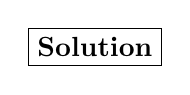
\begin{tikzpicture}
	\node (B) [fill=white,draw] at (2,-2)  {\textbf{Solution}};
	\end{tikzpicture}
	.\\[-0.8cm]
	\def\FrameCommand
	{%
		{\color{purple}\vrule width 3pt}%
		\hspace{0pt}%must no space.
		\fboxsep=\FrameSep\colorbox{mygray}%
	}%
	\MakeFramed{\hsize#1\advance\hsize-\width\FrameRestore}%
	\noindent
}
{\endMakeFramed}





\title{Math Cafe}

\begin{document}

%\begin{comment}
\begin{problem}{29/figs/29_archimedes.png}{Birth of Archimedes}
	Nick and Nikoo know that Archimedes' birthday is one of the following 10 dates, but they forgot which one it is (Khordad, Shahrivar, Azar, and Dey are names of months in Persian calendar):

\begin{itemize}
\item  Khordad 4, Khordad 5, Khordad 8,
\item  Shahrivar 4, Shahrivar 7, 
\item Azar 1, Azar 5,
\item  Dey 1, Dey 2, Dey 8
\end{itemize}

The soul of Archimedes comes back to life and whispers the month of his birthday in Nick's ears and day of his birthday in Nikoo's ear. After this, Nick says: 
\begin{center}
``I don't know Archimedes' birthday, but neither does Nikoo."
\end{center}

After hearing what Nick said, Nikoo responded:

\begin{center}
	``I didn't know when his birthday was previously, but now I know."
\end{center}

Then Nick says:

\begin{center}
	``Now I know too."
\end{center}

When is Archimedes' birthday?\\[0.2cm]

Link to the problem on Twitter:  \url{https://twitter.com/Riazi_Cafe/status/1694967860131729819}\end{problem}
\begin{hint}.
\begin{itemize}
\item What is the probability that a particular non-Club card comes after all the Clubs?
\item How does the final solution relate to the above probability?
\end{itemize}

\end{hint}
\begin{solution}
The answer to question is 11.\\[0.2cm]

To show this, we need to prove two propositions:
The first proposition  is that there is a method for Heshmat that if he colors the balls in such a way, the number of red balls in every ninja path will be at most 11.
The second proposition is that no matter how Hashmat colors the balls, there is a ninja path with at least 11 red balls.
Let us first show the first proposition. Consider the following coloring method:
\begin{center}
\begin{tabular}{c}

line $1 \rightarrow 1$\\

line $2 \rightarrow 1$\\

line $3 \rightarrow 3$\\

line $4 \rightarrow 1$\\

line $5 \rightarrow 3$\\

line $6 \rightarrow 5$\\

line $7 \rightarrow 7$\\

line $8 \rightarrow 1$\\

$\vdots$\\
\end{tabular}
\end{center}
In the above coloring method we iterate over lines and color one ball from each line. We start by coloring the first ball of the first line. From then on, for each next line, we move two balls to the right and color the ball if it exists. Otherwise we continue on by coloring the first ball of the current line and repeat the same process for the next lines. In other words, for each line $2^i$ we color ball number 1, and for lines $2^i +j$ we color ball number $1+2j$ ($j < 2^i$).

Due to our coloring, from each interval of lines
$[1,1], [2,3], [4,7], \ldots, [512,1023], [1024,1369]$
there will be a maximum of one colored ball per ninja path. Thus, no ninja path can have more than 11 red balls.


Next, we show the second proposition. In other words, we show that for every coloring of Heshmat, there is a ninja path for Gholi with at least 11 colored balls.

For this we leverage the Dilworth theorem below:
\begin{theorem}[Dilworth theorem, \url{https://en.wikipedia.org/wiki/Dilworth\%27s_theorem}]
	 In any finite partially ordered set, the largest antichain has the same size as the smallest chain decomposition.
\end{theorem}
The Dilworth theorem shows that if there is no ninja path with 11 red balls for some coloring, then the line can be divided into 10 groups such that no two red balls in lines of a group are reachable from one another. In other words, if lines $i$ and $j$ are in the same group and their red balls are at positions $a$ and $b$, then we have $|a-b| > |i-j|$.  One can see that this is impossible since $2^{10} < 1369$.\end{solution}
\newpage

\begin{problem}{29/figs/29_archimedes.png}{Birth of Archimedes}
	Nick and Nikoo know that Archimedes' birthday is one of the following 10 dates, but they forgot which one it is (Khordad, Shahrivar, Azar, and Dey are names of months in Persian calendar):

\begin{itemize}
\item  Khordad 4, Khordad 5, Khordad 8,
\item  Shahrivar 4, Shahrivar 7, 
\item Azar 1, Azar 5,
\item  Dey 1, Dey 2, Dey 8
\end{itemize}

The soul of Archimedes comes back to life and whispers the month of his birthday in Nick's ears and day of his birthday in Nikoo's ear. After this, Nick says: 
\begin{center}
``I don't know Archimedes' birthday, but neither does Nikoo."
\end{center}

After hearing what Nick said, Nikoo responded:

\begin{center}
	``I didn't know when his birthday was previously, but now I know."
\end{center}

Then Nick says:

\begin{center}
	``Now I know too."
\end{center}

When is Archimedes' birthday?\\[0.2cm]

Link to the problem on Twitter:  \url{https://twitter.com/Riazi_Cafe/status/1694967860131729819}\end{problem}
\begin{solution}
The answer to question is 11.\\[0.2cm]

To show this, we need to prove two propositions:
The first proposition  is that there is a method for Heshmat that if he colors the balls in such a way, the number of red balls in every ninja path will be at most 11.
The second proposition is that no matter how Hashmat colors the balls, there is a ninja path with at least 11 red balls.
Let us first show the first proposition. Consider the following coloring method:
\begin{center}
\begin{tabular}{c}

line $1 \rightarrow 1$\\

line $2 \rightarrow 1$\\

line $3 \rightarrow 3$\\

line $4 \rightarrow 1$\\

line $5 \rightarrow 3$\\

line $6 \rightarrow 5$\\

line $7 \rightarrow 7$\\

line $8 \rightarrow 1$\\

$\vdots$\\
\end{tabular}
\end{center}
In the above coloring method we iterate over lines and color one ball from each line. We start by coloring the first ball of the first line. From then on, for each next line, we move two balls to the right and color the ball if it exists. Otherwise we continue on by coloring the first ball of the current line and repeat the same process for the next lines. In other words, for each line $2^i$ we color ball number 1, and for lines $2^i +j$ we color ball number $1+2j$ ($j < 2^i$).

Due to our coloring, from each interval of lines
$[1,1], [2,3], [4,7], \ldots, [512,1023], [1024,1369]$
there will be a maximum of one colored ball per ninja path. Thus, no ninja path can have more than 11 red balls.


Next, we show the second proposition. In other words, we show that for every coloring of Heshmat, there is a ninja path for Gholi with at least 11 colored balls.

For this we leverage the Dilworth theorem below:
\begin{theorem}[Dilworth theorem, \url{https://en.wikipedia.org/wiki/Dilworth\%27s_theorem}]
	 In any finite partially ordered set, the largest antichain has the same size as the smallest chain decomposition.
\end{theorem}
The Dilworth theorem shows that if there is no ninja path with 11 red balls for some coloring, then the line can be divided into 10 groups such that no two red balls in lines of a group are reachable from one another. In other words, if lines $i$ and $j$ are in the same group and their red balls are at positions $a$ and $b$, then we have $|a-b| > |i-j|$.  One can see that this is impossible since $2^{10} < 1369$.\end{solution}
\newpage

\begin{problem}{29/figs/29_archimedes.png}{Birth of Archimedes}
	Nick and Nikoo know that Archimedes' birthday is one of the following 10 dates, but they forgot which one it is (Khordad, Shahrivar, Azar, and Dey are names of months in Persian calendar):

\begin{itemize}
\item  Khordad 4, Khordad 5, Khordad 8,
\item  Shahrivar 4, Shahrivar 7, 
\item Azar 1, Azar 5,
\item  Dey 1, Dey 2, Dey 8
\end{itemize}

The soul of Archimedes comes back to life and whispers the month of his birthday in Nick's ears and day of his birthday in Nikoo's ear. After this, Nick says: 
\begin{center}
``I don't know Archimedes' birthday, but neither does Nikoo."
\end{center}

After hearing what Nick said, Nikoo responded:

\begin{center}
	``I didn't know when his birthday was previously, but now I know."
\end{center}

Then Nick says:

\begin{center}
	``Now I know too."
\end{center}

When is Archimedes' birthday?\\[0.2cm]

Link to the problem on Twitter:  \url{https://twitter.com/Riazi_Cafe/status/1694967860131729819}\end{problem}
\begin{solution}
The answer to question is 11.\\[0.2cm]

To show this, we need to prove two propositions:
The first proposition  is that there is a method for Heshmat that if he colors the balls in such a way, the number of red balls in every ninja path will be at most 11.
The second proposition is that no matter how Hashmat colors the balls, there is a ninja path with at least 11 red balls.
Let us first show the first proposition. Consider the following coloring method:
\begin{center}
\begin{tabular}{c}

line $1 \rightarrow 1$\\

line $2 \rightarrow 1$\\

line $3 \rightarrow 3$\\

line $4 \rightarrow 1$\\

line $5 \rightarrow 3$\\

line $6 \rightarrow 5$\\

line $7 \rightarrow 7$\\

line $8 \rightarrow 1$\\

$\vdots$\\
\end{tabular}
\end{center}
In the above coloring method we iterate over lines and color one ball from each line. We start by coloring the first ball of the first line. From then on, for each next line, we move two balls to the right and color the ball if it exists. Otherwise we continue on by coloring the first ball of the current line and repeat the same process for the next lines. In other words, for each line $2^i$ we color ball number 1, and for lines $2^i +j$ we color ball number $1+2j$ ($j < 2^i$).

Due to our coloring, from each interval of lines
$[1,1], [2,3], [4,7], \ldots, [512,1023], [1024,1369]$
there will be a maximum of one colored ball per ninja path. Thus, no ninja path can have more than 11 red balls.


Next, we show the second proposition. In other words, we show that for every coloring of Heshmat, there is a ninja path for Gholi with at least 11 colored balls.

For this we leverage the Dilworth theorem below:
\begin{theorem}[Dilworth theorem, \url{https://en.wikipedia.org/wiki/Dilworth\%27s_theorem}]
	 In any finite partially ordered set, the largest antichain has the same size as the smallest chain decomposition.
\end{theorem}
The Dilworth theorem shows that if there is no ninja path with 11 red balls for some coloring, then the line can be divided into 10 groups such that no two red balls in lines of a group are reachable from one another. In other words, if lines $i$ and $j$ are in the same group and their red balls are at positions $a$ and $b$, then we have $|a-b| > |i-j|$.  One can see that this is impossible since $2^{10} < 1369$.\end{solution}
\newpage

\begin{problem}{29/figs/29_archimedes.png}{Birth of Archimedes}
	Nick and Nikoo know that Archimedes' birthday is one of the following 10 dates, but they forgot which one it is (Khordad, Shahrivar, Azar, and Dey are names of months in Persian calendar):

\begin{itemize}
\item  Khordad 4, Khordad 5, Khordad 8,
\item  Shahrivar 4, Shahrivar 7, 
\item Azar 1, Azar 5,
\item  Dey 1, Dey 2, Dey 8
\end{itemize}

The soul of Archimedes comes back to life and whispers the month of his birthday in Nick's ears and day of his birthday in Nikoo's ear. After this, Nick says: 
\begin{center}
``I don't know Archimedes' birthday, but neither does Nikoo."
\end{center}

After hearing what Nick said, Nikoo responded:

\begin{center}
	``I didn't know when his birthday was previously, but now I know."
\end{center}

Then Nick says:

\begin{center}
	``Now I know too."
\end{center}

When is Archimedes' birthday?\\[0.2cm]

Link to the problem on Twitter:  \url{https://twitter.com/Riazi_Cafe/status/1694967860131729819}\end{problem}
\begin{solution}
The answer to question is 11.\\[0.2cm]

To show this, we need to prove two propositions:
The first proposition  is that there is a method for Heshmat that if he colors the balls in such a way, the number of red balls in every ninja path will be at most 11.
The second proposition is that no matter how Hashmat colors the balls, there is a ninja path with at least 11 red balls.
Let us first show the first proposition. Consider the following coloring method:
\begin{center}
\begin{tabular}{c}

line $1 \rightarrow 1$\\

line $2 \rightarrow 1$\\

line $3 \rightarrow 3$\\

line $4 \rightarrow 1$\\

line $5 \rightarrow 3$\\

line $6 \rightarrow 5$\\

line $7 \rightarrow 7$\\

line $8 \rightarrow 1$\\

$\vdots$\\
\end{tabular}
\end{center}
In the above coloring method we iterate over lines and color one ball from each line. We start by coloring the first ball of the first line. From then on, for each next line, we move two balls to the right and color the ball if it exists. Otherwise we continue on by coloring the first ball of the current line and repeat the same process for the next lines. In other words, for each line $2^i$ we color ball number 1, and for lines $2^i +j$ we color ball number $1+2j$ ($j < 2^i$).

Due to our coloring, from each interval of lines
$[1,1], [2,3], [4,7], \ldots, [512,1023], [1024,1369]$
there will be a maximum of one colored ball per ninja path. Thus, no ninja path can have more than 11 red balls.


Next, we show the second proposition. In other words, we show that for every coloring of Heshmat, there is a ninja path for Gholi with at least 11 colored balls.

For this we leverage the Dilworth theorem below:
\begin{theorem}[Dilworth theorem, \url{https://en.wikipedia.org/wiki/Dilworth\%27s_theorem}]
	 In any finite partially ordered set, the largest antichain has the same size as the smallest chain decomposition.
\end{theorem}
The Dilworth theorem shows that if there is no ninja path with 11 red balls for some coloring, then the line can be divided into 10 groups such that no two red balls in lines of a group are reachable from one another. In other words, if lines $i$ and $j$ are in the same group and their red balls are at positions $a$ and $b$, then we have $|a-b| > |i-j|$.  One can see that this is impossible since $2^{10} < 1369$.\end{solution}
\newpage

\begin{problem}{29/figs/29_archimedes.png}{Birth of Archimedes}
	Nick and Nikoo know that Archimedes' birthday is one of the following 10 dates, but they forgot which one it is (Khordad, Shahrivar, Azar, and Dey are names of months in Persian calendar):

\begin{itemize}
\item  Khordad 4, Khordad 5, Khordad 8,
\item  Shahrivar 4, Shahrivar 7, 
\item Azar 1, Azar 5,
\item  Dey 1, Dey 2, Dey 8
\end{itemize}

The soul of Archimedes comes back to life and whispers the month of his birthday in Nick's ears and day of his birthday in Nikoo's ear. After this, Nick says: 
\begin{center}
``I don't know Archimedes' birthday, but neither does Nikoo."
\end{center}

After hearing what Nick said, Nikoo responded:

\begin{center}
	``I didn't know when his birthday was previously, but now I know."
\end{center}

Then Nick says:

\begin{center}
	``Now I know too."
\end{center}

When is Archimedes' birthday?\\[0.2cm]

Link to the problem on Twitter:  \url{https://twitter.com/Riazi_Cafe/status/1694967860131729819}\end{problem}
\begin{solution}
The answer to question is 11.\\[0.2cm]

To show this, we need to prove two propositions:
The first proposition  is that there is a method for Heshmat that if he colors the balls in such a way, the number of red balls in every ninja path will be at most 11.
The second proposition is that no matter how Hashmat colors the balls, there is a ninja path with at least 11 red balls.
Let us first show the first proposition. Consider the following coloring method:
\begin{center}
\begin{tabular}{c}

line $1 \rightarrow 1$\\

line $2 \rightarrow 1$\\

line $3 \rightarrow 3$\\

line $4 \rightarrow 1$\\

line $5 \rightarrow 3$\\

line $6 \rightarrow 5$\\

line $7 \rightarrow 7$\\

line $8 \rightarrow 1$\\

$\vdots$\\
\end{tabular}
\end{center}
In the above coloring method we iterate over lines and color one ball from each line. We start by coloring the first ball of the first line. From then on, for each next line, we move two balls to the right and color the ball if it exists. Otherwise we continue on by coloring the first ball of the current line and repeat the same process for the next lines. In other words, for each line $2^i$ we color ball number 1, and for lines $2^i +j$ we color ball number $1+2j$ ($j < 2^i$).

Due to our coloring, from each interval of lines
$[1,1], [2,3], [4,7], \ldots, [512,1023], [1024,1369]$
there will be a maximum of one colored ball per ninja path. Thus, no ninja path can have more than 11 red balls.


Next, we show the second proposition. In other words, we show that for every coloring of Heshmat, there is a ninja path for Gholi with at least 11 colored balls.

For this we leverage the Dilworth theorem below:
\begin{theorem}[Dilworth theorem, \url{https://en.wikipedia.org/wiki/Dilworth\%27s_theorem}]
	 In any finite partially ordered set, the largest antichain has the same size as the smallest chain decomposition.
\end{theorem}
The Dilworth theorem shows that if there is no ninja path with 11 red balls for some coloring, then the line can be divided into 10 groups such that no two red balls in lines of a group are reachable from one another. In other words, if lines $i$ and $j$ are in the same group and their red balls are at positions $a$ and $b$, then we have $|a-b| > |i-j|$.  One can see that this is impossible since $2^{10} < 1369$.\end{solution}
\newpage

\begin{problem}{29/figs/29_archimedes.png}{Birth of Archimedes}
	Nick and Nikoo know that Archimedes' birthday is one of the following 10 dates, but they forgot which one it is (Khordad, Shahrivar, Azar, and Dey are names of months in Persian calendar):

\begin{itemize}
\item  Khordad 4, Khordad 5, Khordad 8,
\item  Shahrivar 4, Shahrivar 7, 
\item Azar 1, Azar 5,
\item  Dey 1, Dey 2, Dey 8
\end{itemize}

The soul of Archimedes comes back to life and whispers the month of his birthday in Nick's ears and day of his birthday in Nikoo's ear. After this, Nick says: 
\begin{center}
``I don't know Archimedes' birthday, but neither does Nikoo."
\end{center}

After hearing what Nick said, Nikoo responded:

\begin{center}
	``I didn't know when his birthday was previously, but now I know."
\end{center}

Then Nick says:

\begin{center}
	``Now I know too."
\end{center}

When is Archimedes' birthday?\\[0.2cm]

Link to the problem on Twitter:  \url{https://twitter.com/Riazi_Cafe/status/1694967860131729819}\end{problem}
\begin{solution}
The answer to question is 11.\\[0.2cm]

To show this, we need to prove two propositions:
The first proposition  is that there is a method for Heshmat that if he colors the balls in such a way, the number of red balls in every ninja path will be at most 11.
The second proposition is that no matter how Hashmat colors the balls, there is a ninja path with at least 11 red balls.
Let us first show the first proposition. Consider the following coloring method:
\begin{center}
\begin{tabular}{c}

line $1 \rightarrow 1$\\

line $2 \rightarrow 1$\\

line $3 \rightarrow 3$\\

line $4 \rightarrow 1$\\

line $5 \rightarrow 3$\\

line $6 \rightarrow 5$\\

line $7 \rightarrow 7$\\

line $8 \rightarrow 1$\\

$\vdots$\\
\end{tabular}
\end{center}
In the above coloring method we iterate over lines and color one ball from each line. We start by coloring the first ball of the first line. From then on, for each next line, we move two balls to the right and color the ball if it exists. Otherwise we continue on by coloring the first ball of the current line and repeat the same process for the next lines. In other words, for each line $2^i$ we color ball number 1, and for lines $2^i +j$ we color ball number $1+2j$ ($j < 2^i$).

Due to our coloring, from each interval of lines
$[1,1], [2,3], [4,7], \ldots, [512,1023], [1024,1369]$
there will be a maximum of one colored ball per ninja path. Thus, no ninja path can have more than 11 red balls.


Next, we show the second proposition. In other words, we show that for every coloring of Heshmat, there is a ninja path for Gholi with at least 11 colored balls.

For this we leverage the Dilworth theorem below:
\begin{theorem}[Dilworth theorem, \url{https://en.wikipedia.org/wiki/Dilworth\%27s_theorem}]
	 In any finite partially ordered set, the largest antichain has the same size as the smallest chain decomposition.
\end{theorem}
The Dilworth theorem shows that if there is no ninja path with 11 red balls for some coloring, then the line can be divided into 10 groups such that no two red balls in lines of a group are reachable from one another. In other words, if lines $i$ and $j$ are in the same group and their red balls are at positions $a$ and $b$, then we have $|a-b| > |i-j|$.  One can see that this is impossible since $2^{10} < 1369$.\end{solution}
\newpage


\begin{problem}{29/figs/29_archimedes.png}{Birth of Archimedes}
	Nick and Nikoo know that Archimedes' birthday is one of the following 10 dates, but they forgot which one it is (Khordad, Shahrivar, Azar, and Dey are names of months in Persian calendar):

\begin{itemize}
\item  Khordad 4, Khordad 5, Khordad 8,
\item  Shahrivar 4, Shahrivar 7, 
\item Azar 1, Azar 5,
\item  Dey 1, Dey 2, Dey 8
\end{itemize}

The soul of Archimedes comes back to life and whispers the month of his birthday in Nick's ears and day of his birthday in Nikoo's ear. After this, Nick says: 
\begin{center}
``I don't know Archimedes' birthday, but neither does Nikoo."
\end{center}

After hearing what Nick said, Nikoo responded:

\begin{center}
	``I didn't know when his birthday was previously, but now I know."
\end{center}

Then Nick says:

\begin{center}
	``Now I know too."
\end{center}

When is Archimedes' birthday?\\[0.2cm]

Link to the problem on Twitter:  \url{https://twitter.com/Riazi_Cafe/status/1694967860131729819}\end{problem}
\begin{solution}
The answer to question is 11.\\[0.2cm]

To show this, we need to prove two propositions:
The first proposition  is that there is a method for Heshmat that if he colors the balls in such a way, the number of red balls in every ninja path will be at most 11.
The second proposition is that no matter how Hashmat colors the balls, there is a ninja path with at least 11 red balls.
Let us first show the first proposition. Consider the following coloring method:
\begin{center}
\begin{tabular}{c}

line $1 \rightarrow 1$\\

line $2 \rightarrow 1$\\

line $3 \rightarrow 3$\\

line $4 \rightarrow 1$\\

line $5 \rightarrow 3$\\

line $6 \rightarrow 5$\\

line $7 \rightarrow 7$\\

line $8 \rightarrow 1$\\

$\vdots$\\
\end{tabular}
\end{center}
In the above coloring method we iterate over lines and color one ball from each line. We start by coloring the first ball of the first line. From then on, for each next line, we move two balls to the right and color the ball if it exists. Otherwise we continue on by coloring the first ball of the current line and repeat the same process for the next lines. In other words, for each line $2^i$ we color ball number 1, and for lines $2^i +j$ we color ball number $1+2j$ ($j < 2^i$).

Due to our coloring, from each interval of lines
$[1,1], [2,3], [4,7], \ldots, [512,1023], [1024,1369]$
there will be a maximum of one colored ball per ninja path. Thus, no ninja path can have more than 11 red balls.


Next, we show the second proposition. In other words, we show that for every coloring of Heshmat, there is a ninja path for Gholi with at least 11 colored balls.

For this we leverage the Dilworth theorem below:
\begin{theorem}[Dilworth theorem, \url{https://en.wikipedia.org/wiki/Dilworth\%27s_theorem}]
	 In any finite partially ordered set, the largest antichain has the same size as the smallest chain decomposition.
\end{theorem}
The Dilworth theorem shows that if there is no ninja path with 11 red balls for some coloring, then the line can be divided into 10 groups such that no two red balls in lines of a group are reachable from one another. In other words, if lines $i$ and $j$ are in the same group and their red balls are at positions $a$ and $b$, then we have $|a-b| > |i-j|$.  One can see that this is impossible since $2^{10} < 1369$.\end{solution}
\newpage


\begin{problem}{29/figs/29_archimedes.png}{Birth of Archimedes}
	Nick and Nikoo know that Archimedes' birthday is one of the following 10 dates, but they forgot which one it is (Khordad, Shahrivar, Azar, and Dey are names of months in Persian calendar):

\begin{itemize}
\item  Khordad 4, Khordad 5, Khordad 8,
\item  Shahrivar 4, Shahrivar 7, 
\item Azar 1, Azar 5,
\item  Dey 1, Dey 2, Dey 8
\end{itemize}

The soul of Archimedes comes back to life and whispers the month of his birthday in Nick's ears and day of his birthday in Nikoo's ear. After this, Nick says: 
\begin{center}
``I don't know Archimedes' birthday, but neither does Nikoo."
\end{center}

After hearing what Nick said, Nikoo responded:

\begin{center}
	``I didn't know when his birthday was previously, but now I know."
\end{center}

Then Nick says:

\begin{center}
	``Now I know too."
\end{center}

When is Archimedes' birthday?\\[0.2cm]

Link to the problem on Twitter:  \url{https://twitter.com/Riazi_Cafe/status/1694967860131729819}\end{problem}
\begin{solution}
The answer to question is 11.\\[0.2cm]

To show this, we need to prove two propositions:
The first proposition  is that there is a method for Heshmat that if he colors the balls in such a way, the number of red balls in every ninja path will be at most 11.
The second proposition is that no matter how Hashmat colors the balls, there is a ninja path with at least 11 red balls.
Let us first show the first proposition. Consider the following coloring method:
\begin{center}
\begin{tabular}{c}

line $1 \rightarrow 1$\\

line $2 \rightarrow 1$\\

line $3 \rightarrow 3$\\

line $4 \rightarrow 1$\\

line $5 \rightarrow 3$\\

line $6 \rightarrow 5$\\

line $7 \rightarrow 7$\\

line $8 \rightarrow 1$\\

$\vdots$\\
\end{tabular}
\end{center}
In the above coloring method we iterate over lines and color one ball from each line. We start by coloring the first ball of the first line. From then on, for each next line, we move two balls to the right and color the ball if it exists. Otherwise we continue on by coloring the first ball of the current line and repeat the same process for the next lines. In other words, for each line $2^i$ we color ball number 1, and for lines $2^i +j$ we color ball number $1+2j$ ($j < 2^i$).

Due to our coloring, from each interval of lines
$[1,1], [2,3], [4,7], \ldots, [512,1023], [1024,1369]$
there will be a maximum of one colored ball per ninja path. Thus, no ninja path can have more than 11 red balls.


Next, we show the second proposition. In other words, we show that for every coloring of Heshmat, there is a ninja path for Gholi with at least 11 colored balls.

For this we leverage the Dilworth theorem below:
\begin{theorem}[Dilworth theorem, \url{https://en.wikipedia.org/wiki/Dilworth\%27s_theorem}]
	 In any finite partially ordered set, the largest antichain has the same size as the smallest chain decomposition.
\end{theorem}
The Dilworth theorem shows that if there is no ninja path with 11 red balls for some coloring, then the line can be divided into 10 groups such that no two red balls in lines of a group are reachable from one another. In other words, if lines $i$ and $j$ are in the same group and their red balls are at positions $a$ and $b$, then we have $|a-b| > |i-j|$.  One can see that this is impossible since $2^{10} < 1369$.\end{solution}
\newpage


\begin{problem}{29/figs/29_archimedes.png}{Birth of Archimedes}
	Nick and Nikoo know that Archimedes' birthday is one of the following 10 dates, but they forgot which one it is (Khordad, Shahrivar, Azar, and Dey are names of months in Persian calendar):

\begin{itemize}
\item  Khordad 4, Khordad 5, Khordad 8,
\item  Shahrivar 4, Shahrivar 7, 
\item Azar 1, Azar 5,
\item  Dey 1, Dey 2, Dey 8
\end{itemize}

The soul of Archimedes comes back to life and whispers the month of his birthday in Nick's ears and day of his birthday in Nikoo's ear. After this, Nick says: 
\begin{center}
``I don't know Archimedes' birthday, but neither does Nikoo."
\end{center}

After hearing what Nick said, Nikoo responded:

\begin{center}
	``I didn't know when his birthday was previously, but now I know."
\end{center}

Then Nick says:

\begin{center}
	``Now I know too."
\end{center}

When is Archimedes' birthday?\\[0.2cm]

Link to the problem on Twitter:  \url{https://twitter.com/Riazi_Cafe/status/1694967860131729819}\end{problem}
\begin{solution}
The answer to question is 11.\\[0.2cm]

To show this, we need to prove two propositions:
The first proposition  is that there is a method for Heshmat that if he colors the balls in such a way, the number of red balls in every ninja path will be at most 11.
The second proposition is that no matter how Hashmat colors the balls, there is a ninja path with at least 11 red balls.
Let us first show the first proposition. Consider the following coloring method:
\begin{center}
\begin{tabular}{c}

line $1 \rightarrow 1$\\

line $2 \rightarrow 1$\\

line $3 \rightarrow 3$\\

line $4 \rightarrow 1$\\

line $5 \rightarrow 3$\\

line $6 \rightarrow 5$\\

line $7 \rightarrow 7$\\

line $8 \rightarrow 1$\\

$\vdots$\\
\end{tabular}
\end{center}
In the above coloring method we iterate over lines and color one ball from each line. We start by coloring the first ball of the first line. From then on, for each next line, we move two balls to the right and color the ball if it exists. Otherwise we continue on by coloring the first ball of the current line and repeat the same process for the next lines. In other words, for each line $2^i$ we color ball number 1, and for lines $2^i +j$ we color ball number $1+2j$ ($j < 2^i$).

Due to our coloring, from each interval of lines
$[1,1], [2,3], [4,7], \ldots, [512,1023], [1024,1369]$
there will be a maximum of one colored ball per ninja path. Thus, no ninja path can have more than 11 red balls.


Next, we show the second proposition. In other words, we show that for every coloring of Heshmat, there is a ninja path for Gholi with at least 11 colored balls.

For this we leverage the Dilworth theorem below:
\begin{theorem}[Dilworth theorem, \url{https://en.wikipedia.org/wiki/Dilworth\%27s_theorem}]
	 In any finite partially ordered set, the largest antichain has the same size as the smallest chain decomposition.
\end{theorem}
The Dilworth theorem shows that if there is no ninja path with 11 red balls for some coloring, then the line can be divided into 10 groups such that no two red balls in lines of a group are reachable from one another. In other words, if lines $i$ and $j$ are in the same group and their red balls are at positions $a$ and $b$, then we have $|a-b| > |i-j|$.  One can see that this is impossible since $2^{10} < 1369$.\end{solution}
\newpage

\begin{problem}{29/figs/29_archimedes.png}{Birth of Archimedes}
	Nick and Nikoo know that Archimedes' birthday is one of the following 10 dates, but they forgot which one it is (Khordad, Shahrivar, Azar, and Dey are names of months in Persian calendar):

\begin{itemize}
\item  Khordad 4, Khordad 5, Khordad 8,
\item  Shahrivar 4, Shahrivar 7, 
\item Azar 1, Azar 5,
\item  Dey 1, Dey 2, Dey 8
\end{itemize}

The soul of Archimedes comes back to life and whispers the month of his birthday in Nick's ears and day of his birthday in Nikoo's ear. After this, Nick says: 
\begin{center}
``I don't know Archimedes' birthday, but neither does Nikoo."
\end{center}

After hearing what Nick said, Nikoo responded:

\begin{center}
	``I didn't know when his birthday was previously, but now I know."
\end{center}

Then Nick says:

\begin{center}
	``Now I know too."
\end{center}

When is Archimedes' birthday?\\[0.2cm]

Link to the problem on Twitter:  \url{https://twitter.com/Riazi_Cafe/status/1694967860131729819}\end{problem}
\begin{solution}
The answer to question is 11.\\[0.2cm]

To show this, we need to prove two propositions:
The first proposition  is that there is a method for Heshmat that if he colors the balls in such a way, the number of red balls in every ninja path will be at most 11.
The second proposition is that no matter how Hashmat colors the balls, there is a ninja path with at least 11 red balls.
Let us first show the first proposition. Consider the following coloring method:
\begin{center}
\begin{tabular}{c}

line $1 \rightarrow 1$\\

line $2 \rightarrow 1$\\

line $3 \rightarrow 3$\\

line $4 \rightarrow 1$\\

line $5 \rightarrow 3$\\

line $6 \rightarrow 5$\\

line $7 \rightarrow 7$\\

line $8 \rightarrow 1$\\

$\vdots$\\
\end{tabular}
\end{center}
In the above coloring method we iterate over lines and color one ball from each line. We start by coloring the first ball of the first line. From then on, for each next line, we move two balls to the right and color the ball if it exists. Otherwise we continue on by coloring the first ball of the current line and repeat the same process for the next lines. In other words, for each line $2^i$ we color ball number 1, and for lines $2^i +j$ we color ball number $1+2j$ ($j < 2^i$).

Due to our coloring, from each interval of lines
$[1,1], [2,3], [4,7], \ldots, [512,1023], [1024,1369]$
there will be a maximum of one colored ball per ninja path. Thus, no ninja path can have more than 11 red balls.


Next, we show the second proposition. In other words, we show that for every coloring of Heshmat, there is a ninja path for Gholi with at least 11 colored balls.

For this we leverage the Dilworth theorem below:
\begin{theorem}[Dilworth theorem, \url{https://en.wikipedia.org/wiki/Dilworth\%27s_theorem}]
	 In any finite partially ordered set, the largest antichain has the same size as the smallest chain decomposition.
\end{theorem}
The Dilworth theorem shows that if there is no ninja path with 11 red balls for some coloring, then the line can be divided into 10 groups such that no two red balls in lines of a group are reachable from one another. In other words, if lines $i$ and $j$ are in the same group and their red balls are at positions $a$ and $b$, then we have $|a-b| > |i-j|$.  One can see that this is impossible since $2^{10} < 1369$.\end{solution}
\newpage


\begin{problem}{29/figs/29_archimedes.png}{Birth of Archimedes}
	Nick and Nikoo know that Archimedes' birthday is one of the following 10 dates, but they forgot which one it is (Khordad, Shahrivar, Azar, and Dey are names of months in Persian calendar):

\begin{itemize}
\item  Khordad 4, Khordad 5, Khordad 8,
\item  Shahrivar 4, Shahrivar 7, 
\item Azar 1, Azar 5,
\item  Dey 1, Dey 2, Dey 8
\end{itemize}

The soul of Archimedes comes back to life and whispers the month of his birthday in Nick's ears and day of his birthday in Nikoo's ear. After this, Nick says: 
\begin{center}
``I don't know Archimedes' birthday, but neither does Nikoo."
\end{center}

After hearing what Nick said, Nikoo responded:

\begin{center}
	``I didn't know when his birthday was previously, but now I know."
\end{center}

Then Nick says:

\begin{center}
	``Now I know too."
\end{center}

When is Archimedes' birthday?\\[0.2cm]

Link to the problem on Twitter:  \url{https://twitter.com/Riazi_Cafe/status/1694967860131729819}\end{problem}
\begin{solution}
The answer to question is 11.\\[0.2cm]

To show this, we need to prove two propositions:
The first proposition  is that there is a method for Heshmat that if he colors the balls in such a way, the number of red balls in every ninja path will be at most 11.
The second proposition is that no matter how Hashmat colors the balls, there is a ninja path with at least 11 red balls.
Let us first show the first proposition. Consider the following coloring method:
\begin{center}
\begin{tabular}{c}

line $1 \rightarrow 1$\\

line $2 \rightarrow 1$\\

line $3 \rightarrow 3$\\

line $4 \rightarrow 1$\\

line $5 \rightarrow 3$\\

line $6 \rightarrow 5$\\

line $7 \rightarrow 7$\\

line $8 \rightarrow 1$\\

$\vdots$\\
\end{tabular}
\end{center}
In the above coloring method we iterate over lines and color one ball from each line. We start by coloring the first ball of the first line. From then on, for each next line, we move two balls to the right and color the ball if it exists. Otherwise we continue on by coloring the first ball of the current line and repeat the same process for the next lines. In other words, for each line $2^i$ we color ball number 1, and for lines $2^i +j$ we color ball number $1+2j$ ($j < 2^i$).

Due to our coloring, from each interval of lines
$[1,1], [2,3], [4,7], \ldots, [512,1023], [1024,1369]$
there will be a maximum of one colored ball per ninja path. Thus, no ninja path can have more than 11 red balls.


Next, we show the second proposition. In other words, we show that for every coloring of Heshmat, there is a ninja path for Gholi with at least 11 colored balls.

For this we leverage the Dilworth theorem below:
\begin{theorem}[Dilworth theorem, \url{https://en.wikipedia.org/wiki/Dilworth\%27s_theorem}]
	 In any finite partially ordered set, the largest antichain has the same size as the smallest chain decomposition.
\end{theorem}
The Dilworth theorem shows that if there is no ninja path with 11 red balls for some coloring, then the line can be divided into 10 groups such that no two red balls in lines of a group are reachable from one another. In other words, if lines $i$ and $j$ are in the same group and their red balls are at positions $a$ and $b$, then we have $|a-b| > |i-j|$.  One can see that this is impossible since $2^{10} < 1369$.\end{solution}
\newpage


\begin{problem}{29/figs/29_archimedes.png}{Birth of Archimedes}
	Nick and Nikoo know that Archimedes' birthday is one of the following 10 dates, but they forgot which one it is (Khordad, Shahrivar, Azar, and Dey are names of months in Persian calendar):

\begin{itemize}
\item  Khordad 4, Khordad 5, Khordad 8,
\item  Shahrivar 4, Shahrivar 7, 
\item Azar 1, Azar 5,
\item  Dey 1, Dey 2, Dey 8
\end{itemize}

The soul of Archimedes comes back to life and whispers the month of his birthday in Nick's ears and day of his birthday in Nikoo's ear. After this, Nick says: 
\begin{center}
``I don't know Archimedes' birthday, but neither does Nikoo."
\end{center}

After hearing what Nick said, Nikoo responded:

\begin{center}
	``I didn't know when his birthday was previously, but now I know."
\end{center}

Then Nick says:

\begin{center}
	``Now I know too."
\end{center}

When is Archimedes' birthday?\\[0.2cm]

Link to the problem on Twitter:  \url{https://twitter.com/Riazi_Cafe/status/1694967860131729819}\end{problem}
\begin{solution}
The answer to question is 11.\\[0.2cm]

To show this, we need to prove two propositions:
The first proposition  is that there is a method for Heshmat that if he colors the balls in such a way, the number of red balls in every ninja path will be at most 11.
The second proposition is that no matter how Hashmat colors the balls, there is a ninja path with at least 11 red balls.
Let us first show the first proposition. Consider the following coloring method:
\begin{center}
\begin{tabular}{c}

line $1 \rightarrow 1$\\

line $2 \rightarrow 1$\\

line $3 \rightarrow 3$\\

line $4 \rightarrow 1$\\

line $5 \rightarrow 3$\\

line $6 \rightarrow 5$\\

line $7 \rightarrow 7$\\

line $8 \rightarrow 1$\\

$\vdots$\\
\end{tabular}
\end{center}
In the above coloring method we iterate over lines and color one ball from each line. We start by coloring the first ball of the first line. From then on, for each next line, we move two balls to the right and color the ball if it exists. Otherwise we continue on by coloring the first ball of the current line and repeat the same process for the next lines. In other words, for each line $2^i$ we color ball number 1, and for lines $2^i +j$ we color ball number $1+2j$ ($j < 2^i$).

Due to our coloring, from each interval of lines
$[1,1], [2,3], [4,7], \ldots, [512,1023], [1024,1369]$
there will be a maximum of one colored ball per ninja path. Thus, no ninja path can have more than 11 red balls.


Next, we show the second proposition. In other words, we show that for every coloring of Heshmat, there is a ninja path for Gholi with at least 11 colored balls.

For this we leverage the Dilworth theorem below:
\begin{theorem}[Dilworth theorem, \url{https://en.wikipedia.org/wiki/Dilworth\%27s_theorem}]
	 In any finite partially ordered set, the largest antichain has the same size as the smallest chain decomposition.
\end{theorem}
The Dilworth theorem shows that if there is no ninja path with 11 red balls for some coloring, then the line can be divided into 10 groups such that no two red balls in lines of a group are reachable from one another. In other words, if lines $i$ and $j$ are in the same group and their red balls are at positions $a$ and $b$, then we have $|a-b| > |i-j|$.  One can see that this is impossible since $2^{10} < 1369$.\end{solution}
\newpage


\begin{problem}{29/figs/29_archimedes.png}{Birth of Archimedes}
	Nick and Nikoo know that Archimedes' birthday is one of the following 10 dates, but they forgot which one it is (Khordad, Shahrivar, Azar, and Dey are names of months in Persian calendar):

\begin{itemize}
\item  Khordad 4, Khordad 5, Khordad 8,
\item  Shahrivar 4, Shahrivar 7, 
\item Azar 1, Azar 5,
\item  Dey 1, Dey 2, Dey 8
\end{itemize}

The soul of Archimedes comes back to life and whispers the month of his birthday in Nick's ears and day of his birthday in Nikoo's ear. After this, Nick says: 
\begin{center}
``I don't know Archimedes' birthday, but neither does Nikoo."
\end{center}

After hearing what Nick said, Nikoo responded:

\begin{center}
	``I didn't know when his birthday was previously, but now I know."
\end{center}

Then Nick says:

\begin{center}
	``Now I know too."
\end{center}

When is Archimedes' birthday?\\[0.2cm]

Link to the problem on Twitter:  \url{https://twitter.com/Riazi_Cafe/status/1694967860131729819}\end{problem}
\begin{solution}
The answer to question is 11.\\[0.2cm]

To show this, we need to prove two propositions:
The first proposition  is that there is a method for Heshmat that if he colors the balls in such a way, the number of red balls in every ninja path will be at most 11.
The second proposition is that no matter how Hashmat colors the balls, there is a ninja path with at least 11 red balls.
Let us first show the first proposition. Consider the following coloring method:
\begin{center}
\begin{tabular}{c}

line $1 \rightarrow 1$\\

line $2 \rightarrow 1$\\

line $3 \rightarrow 3$\\

line $4 \rightarrow 1$\\

line $5 \rightarrow 3$\\

line $6 \rightarrow 5$\\

line $7 \rightarrow 7$\\

line $8 \rightarrow 1$\\

$\vdots$\\
\end{tabular}
\end{center}
In the above coloring method we iterate over lines and color one ball from each line. We start by coloring the first ball of the first line. From then on, for each next line, we move two balls to the right and color the ball if it exists. Otherwise we continue on by coloring the first ball of the current line and repeat the same process for the next lines. In other words, for each line $2^i$ we color ball number 1, and for lines $2^i +j$ we color ball number $1+2j$ ($j < 2^i$).

Due to our coloring, from each interval of lines
$[1,1], [2,3], [4,7], \ldots, [512,1023], [1024,1369]$
there will be a maximum of one colored ball per ninja path. Thus, no ninja path can have more than 11 red balls.


Next, we show the second proposition. In other words, we show that for every coloring of Heshmat, there is a ninja path for Gholi with at least 11 colored balls.

For this we leverage the Dilworth theorem below:
\begin{theorem}[Dilworth theorem, \url{https://en.wikipedia.org/wiki/Dilworth\%27s_theorem}]
	 In any finite partially ordered set, the largest antichain has the same size as the smallest chain decomposition.
\end{theorem}
The Dilworth theorem shows that if there is no ninja path with 11 red balls for some coloring, then the line can be divided into 10 groups such that no two red balls in lines of a group are reachable from one another. In other words, if lines $i$ and $j$ are in the same group and their red balls are at positions $a$ and $b$, then we have $|a-b| > |i-j|$.  One can see that this is impossible since $2^{10} < 1369$.\end{solution}
\newpage


\begin{problem}{29/figs/29_archimedes.png}{Birth of Archimedes}
	Nick and Nikoo know that Archimedes' birthday is one of the following 10 dates, but they forgot which one it is (Khordad, Shahrivar, Azar, and Dey are names of months in Persian calendar):

\begin{itemize}
\item  Khordad 4, Khordad 5, Khordad 8,
\item  Shahrivar 4, Shahrivar 7, 
\item Azar 1, Azar 5,
\item  Dey 1, Dey 2, Dey 8
\end{itemize}

The soul of Archimedes comes back to life and whispers the month of his birthday in Nick's ears and day of his birthday in Nikoo's ear. After this, Nick says: 
\begin{center}
``I don't know Archimedes' birthday, but neither does Nikoo."
\end{center}

After hearing what Nick said, Nikoo responded:

\begin{center}
	``I didn't know when his birthday was previously, but now I know."
\end{center}

Then Nick says:

\begin{center}
	``Now I know too."
\end{center}

When is Archimedes' birthday?\\[0.2cm]

Link to the problem on Twitter:  \url{https://twitter.com/Riazi_Cafe/status/1694967860131729819}\end{problem}
\begin{solution}
The answer to question is 11.\\[0.2cm]

To show this, we need to prove two propositions:
The first proposition  is that there is a method for Heshmat that if he colors the balls in such a way, the number of red balls in every ninja path will be at most 11.
The second proposition is that no matter how Hashmat colors the balls, there is a ninja path with at least 11 red balls.
Let us first show the first proposition. Consider the following coloring method:
\begin{center}
\begin{tabular}{c}

line $1 \rightarrow 1$\\

line $2 \rightarrow 1$\\

line $3 \rightarrow 3$\\

line $4 \rightarrow 1$\\

line $5 \rightarrow 3$\\

line $6 \rightarrow 5$\\

line $7 \rightarrow 7$\\

line $8 \rightarrow 1$\\

$\vdots$\\
\end{tabular}
\end{center}
In the above coloring method we iterate over lines and color one ball from each line. We start by coloring the first ball of the first line. From then on, for each next line, we move two balls to the right and color the ball if it exists. Otherwise we continue on by coloring the first ball of the current line and repeat the same process for the next lines. In other words, for each line $2^i$ we color ball number 1, and for lines $2^i +j$ we color ball number $1+2j$ ($j < 2^i$).

Due to our coloring, from each interval of lines
$[1,1], [2,3], [4,7], \ldots, [512,1023], [1024,1369]$
there will be a maximum of one colored ball per ninja path. Thus, no ninja path can have more than 11 red balls.


Next, we show the second proposition. In other words, we show that for every coloring of Heshmat, there is a ninja path for Gholi with at least 11 colored balls.

For this we leverage the Dilworth theorem below:
\begin{theorem}[Dilworth theorem, \url{https://en.wikipedia.org/wiki/Dilworth\%27s_theorem}]
	 In any finite partially ordered set, the largest antichain has the same size as the smallest chain decomposition.
\end{theorem}
The Dilworth theorem shows that if there is no ninja path with 11 red balls for some coloring, then the line can be divided into 10 groups such that no two red balls in lines of a group are reachable from one another. In other words, if lines $i$ and $j$ are in the same group and their red balls are at positions $a$ and $b$, then we have $|a-b| > |i-j|$.  One can see that this is impossible since $2^{10} < 1369$.\end{solution}
\newpage


\begin{problem}{29/figs/29_archimedes.png}{Birth of Archimedes}
	Nick and Nikoo know that Archimedes' birthday is one of the following 10 dates, but they forgot which one it is (Khordad, Shahrivar, Azar, and Dey are names of months in Persian calendar):

\begin{itemize}
\item  Khordad 4, Khordad 5, Khordad 8,
\item  Shahrivar 4, Shahrivar 7, 
\item Azar 1, Azar 5,
\item  Dey 1, Dey 2, Dey 8
\end{itemize}

The soul of Archimedes comes back to life and whispers the month of his birthday in Nick's ears and day of his birthday in Nikoo's ear. After this, Nick says: 
\begin{center}
``I don't know Archimedes' birthday, but neither does Nikoo."
\end{center}

After hearing what Nick said, Nikoo responded:

\begin{center}
	``I didn't know when his birthday was previously, but now I know."
\end{center}

Then Nick says:

\begin{center}
	``Now I know too."
\end{center}

When is Archimedes' birthday?\\[0.2cm]

Link to the problem on Twitter:  \url{https://twitter.com/Riazi_Cafe/status/1694967860131729819}\end{problem}
\begin{solution}
The answer to question is 11.\\[0.2cm]

To show this, we need to prove two propositions:
The first proposition  is that there is a method for Heshmat that if he colors the balls in such a way, the number of red balls in every ninja path will be at most 11.
The second proposition is that no matter how Hashmat colors the balls, there is a ninja path with at least 11 red balls.
Let us first show the first proposition. Consider the following coloring method:
\begin{center}
\begin{tabular}{c}

line $1 \rightarrow 1$\\

line $2 \rightarrow 1$\\

line $3 \rightarrow 3$\\

line $4 \rightarrow 1$\\

line $5 \rightarrow 3$\\

line $6 \rightarrow 5$\\

line $7 \rightarrow 7$\\

line $8 \rightarrow 1$\\

$\vdots$\\
\end{tabular}
\end{center}
In the above coloring method we iterate over lines and color one ball from each line. We start by coloring the first ball of the first line. From then on, for each next line, we move two balls to the right and color the ball if it exists. Otherwise we continue on by coloring the first ball of the current line and repeat the same process for the next lines. In other words, for each line $2^i$ we color ball number 1, and for lines $2^i +j$ we color ball number $1+2j$ ($j < 2^i$).

Due to our coloring, from each interval of lines
$[1,1], [2,3], [4,7], \ldots, [512,1023], [1024,1369]$
there will be a maximum of one colored ball per ninja path. Thus, no ninja path can have more than 11 red balls.


Next, we show the second proposition. In other words, we show that for every coloring of Heshmat, there is a ninja path for Gholi with at least 11 colored balls.

For this we leverage the Dilworth theorem below:
\begin{theorem}[Dilworth theorem, \url{https://en.wikipedia.org/wiki/Dilworth\%27s_theorem}]
	 In any finite partially ordered set, the largest antichain has the same size as the smallest chain decomposition.
\end{theorem}
The Dilworth theorem shows that if there is no ninja path with 11 red balls for some coloring, then the line can be divided into 10 groups such that no two red balls in lines of a group are reachable from one another. In other words, if lines $i$ and $j$ are in the same group and their red balls are at positions $a$ and $b$, then we have $|a-b| > |i-j|$.  One can see that this is impossible since $2^{10} < 1369$.\end{solution}
\newpage



\begin{problem}{29/figs/29_archimedes.png}{Birth of Archimedes}
	Nick and Nikoo know that Archimedes' birthday is one of the following 10 dates, but they forgot which one it is (Khordad, Shahrivar, Azar, and Dey are names of months in Persian calendar):

\begin{itemize}
\item  Khordad 4, Khordad 5, Khordad 8,
\item  Shahrivar 4, Shahrivar 7, 
\item Azar 1, Azar 5,
\item  Dey 1, Dey 2, Dey 8
\end{itemize}

The soul of Archimedes comes back to life and whispers the month of his birthday in Nick's ears and day of his birthday in Nikoo's ear. After this, Nick says: 
\begin{center}
``I don't know Archimedes' birthday, but neither does Nikoo."
\end{center}

After hearing what Nick said, Nikoo responded:

\begin{center}
	``I didn't know when his birthday was previously, but now I know."
\end{center}

Then Nick says:

\begin{center}
	``Now I know too."
\end{center}

When is Archimedes' birthday?\\[0.2cm]

Link to the problem on Twitter:  \url{https://twitter.com/Riazi_Cafe/status/1694967860131729819}\end{problem}
\begin{solution}
The answer to question is 11.\\[0.2cm]

To show this, we need to prove two propositions:
The first proposition  is that there is a method for Heshmat that if he colors the balls in such a way, the number of red balls in every ninja path will be at most 11.
The second proposition is that no matter how Hashmat colors the balls, there is a ninja path with at least 11 red balls.
Let us first show the first proposition. Consider the following coloring method:
\begin{center}
\begin{tabular}{c}

line $1 \rightarrow 1$\\

line $2 \rightarrow 1$\\

line $3 \rightarrow 3$\\

line $4 \rightarrow 1$\\

line $5 \rightarrow 3$\\

line $6 \rightarrow 5$\\

line $7 \rightarrow 7$\\

line $8 \rightarrow 1$\\

$\vdots$\\
\end{tabular}
\end{center}
In the above coloring method we iterate over lines and color one ball from each line. We start by coloring the first ball of the first line. From then on, for each next line, we move two balls to the right and color the ball if it exists. Otherwise we continue on by coloring the first ball of the current line and repeat the same process for the next lines. In other words, for each line $2^i$ we color ball number 1, and for lines $2^i +j$ we color ball number $1+2j$ ($j < 2^i$).

Due to our coloring, from each interval of lines
$[1,1], [2,3], [4,7], \ldots, [512,1023], [1024,1369]$
there will be a maximum of one colored ball per ninja path. Thus, no ninja path can have more than 11 red balls.


Next, we show the second proposition. In other words, we show that for every coloring of Heshmat, there is a ninja path for Gholi with at least 11 colored balls.

For this we leverage the Dilworth theorem below:
\begin{theorem}[Dilworth theorem, \url{https://en.wikipedia.org/wiki/Dilworth\%27s_theorem}]
	 In any finite partially ordered set, the largest antichain has the same size as the smallest chain decomposition.
\end{theorem}
The Dilworth theorem shows that if there is no ninja path with 11 red balls for some coloring, then the line can be divided into 10 groups such that no two red balls in lines of a group are reachable from one another. In other words, if lines $i$ and $j$ are in the same group and their red balls are at positions $a$ and $b$, then we have $|a-b| > |i-j|$.  One can see that this is impossible since $2^{10} < 1369$.\end{solution}
\newpage


\begin{problem}{29/figs/29_archimedes.png}{Birth of Archimedes}
	Nick and Nikoo know that Archimedes' birthday is one of the following 10 dates, but they forgot which one it is (Khordad, Shahrivar, Azar, and Dey are names of months in Persian calendar):

\begin{itemize}
\item  Khordad 4, Khordad 5, Khordad 8,
\item  Shahrivar 4, Shahrivar 7, 
\item Azar 1, Azar 5,
\item  Dey 1, Dey 2, Dey 8
\end{itemize}

The soul of Archimedes comes back to life and whispers the month of his birthday in Nick's ears and day of his birthday in Nikoo's ear. After this, Nick says: 
\begin{center}
``I don't know Archimedes' birthday, but neither does Nikoo."
\end{center}

After hearing what Nick said, Nikoo responded:

\begin{center}
	``I didn't know when his birthday was previously, but now I know."
\end{center}

Then Nick says:

\begin{center}
	``Now I know too."
\end{center}

When is Archimedes' birthday?\\[0.2cm]

Link to the problem on Twitter:  \url{https://twitter.com/Riazi_Cafe/status/1694967860131729819}\end{problem}
\begin{hint}.
\begin{itemize}
\item What is the probability that a particular non-Club card comes after all the Clubs?
\item How does the final solution relate to the above probability?
\end{itemize}

\end{hint}
\begin{solution}
The answer to question is 11.\\[0.2cm]

To show this, we need to prove two propositions:
The first proposition  is that there is a method for Heshmat that if he colors the balls in such a way, the number of red balls in every ninja path will be at most 11.
The second proposition is that no matter how Hashmat colors the balls, there is a ninja path with at least 11 red balls.
Let us first show the first proposition. Consider the following coloring method:
\begin{center}
\begin{tabular}{c}

line $1 \rightarrow 1$\\

line $2 \rightarrow 1$\\

line $3 \rightarrow 3$\\

line $4 \rightarrow 1$\\

line $5 \rightarrow 3$\\

line $6 \rightarrow 5$\\

line $7 \rightarrow 7$\\

line $8 \rightarrow 1$\\

$\vdots$\\
\end{tabular}
\end{center}
In the above coloring method we iterate over lines and color one ball from each line. We start by coloring the first ball of the first line. From then on, for each next line, we move two balls to the right and color the ball if it exists. Otherwise we continue on by coloring the first ball of the current line and repeat the same process for the next lines. In other words, for each line $2^i$ we color ball number 1, and for lines $2^i +j$ we color ball number $1+2j$ ($j < 2^i$).

Due to our coloring, from each interval of lines
$[1,1], [2,3], [4,7], \ldots, [512,1023], [1024,1369]$
there will be a maximum of one colored ball per ninja path. Thus, no ninja path can have more than 11 red balls.


Next, we show the second proposition. In other words, we show that for every coloring of Heshmat, there is a ninja path for Gholi with at least 11 colored balls.

For this we leverage the Dilworth theorem below:
\begin{theorem}[Dilworth theorem, \url{https://en.wikipedia.org/wiki/Dilworth\%27s_theorem}]
	 In any finite partially ordered set, the largest antichain has the same size as the smallest chain decomposition.
\end{theorem}
The Dilworth theorem shows that if there is no ninja path with 11 red balls for some coloring, then the line can be divided into 10 groups such that no two red balls in lines of a group are reachable from one another. In other words, if lines $i$ and $j$ are in the same group and their red balls are at positions $a$ and $b$, then we have $|a-b| > |i-j|$.  One can see that this is impossible since $2^{10} < 1369$.\end{solution}
\newpage


\begin{problem}{29/figs/29_archimedes.png}{Birth of Archimedes}
	Nick and Nikoo know that Archimedes' birthday is one of the following 10 dates, but they forgot which one it is (Khordad, Shahrivar, Azar, and Dey are names of months in Persian calendar):

\begin{itemize}
\item  Khordad 4, Khordad 5, Khordad 8,
\item  Shahrivar 4, Shahrivar 7, 
\item Azar 1, Azar 5,
\item  Dey 1, Dey 2, Dey 8
\end{itemize}

The soul of Archimedes comes back to life and whispers the month of his birthday in Nick's ears and day of his birthday in Nikoo's ear. After this, Nick says: 
\begin{center}
``I don't know Archimedes' birthday, but neither does Nikoo."
\end{center}

After hearing what Nick said, Nikoo responded:

\begin{center}
	``I didn't know when his birthday was previously, but now I know."
\end{center}

Then Nick says:

\begin{center}
	``Now I know too."
\end{center}

When is Archimedes' birthday?\\[0.2cm]

Link to the problem on Twitter:  \url{https://twitter.com/Riazi_Cafe/status/1694967860131729819}\end{problem}
\begin{solution}
The answer to question is 11.\\[0.2cm]

To show this, we need to prove two propositions:
The first proposition  is that there is a method for Heshmat that if he colors the balls in such a way, the number of red balls in every ninja path will be at most 11.
The second proposition is that no matter how Hashmat colors the balls, there is a ninja path with at least 11 red balls.
Let us first show the first proposition. Consider the following coloring method:
\begin{center}
\begin{tabular}{c}

line $1 \rightarrow 1$\\

line $2 \rightarrow 1$\\

line $3 \rightarrow 3$\\

line $4 \rightarrow 1$\\

line $5 \rightarrow 3$\\

line $6 \rightarrow 5$\\

line $7 \rightarrow 7$\\

line $8 \rightarrow 1$\\

$\vdots$\\
\end{tabular}
\end{center}
In the above coloring method we iterate over lines and color one ball from each line. We start by coloring the first ball of the first line. From then on, for each next line, we move two balls to the right and color the ball if it exists. Otherwise we continue on by coloring the first ball of the current line and repeat the same process for the next lines. In other words, for each line $2^i$ we color ball number 1, and for lines $2^i +j$ we color ball number $1+2j$ ($j < 2^i$).

Due to our coloring, from each interval of lines
$[1,1], [2,3], [4,7], \ldots, [512,1023], [1024,1369]$
there will be a maximum of one colored ball per ninja path. Thus, no ninja path can have more than 11 red balls.


Next, we show the second proposition. In other words, we show that for every coloring of Heshmat, there is a ninja path for Gholi with at least 11 colored balls.

For this we leverage the Dilworth theorem below:
\begin{theorem}[Dilworth theorem, \url{https://en.wikipedia.org/wiki/Dilworth\%27s_theorem}]
	 In any finite partially ordered set, the largest antichain has the same size as the smallest chain decomposition.
\end{theorem}
The Dilworth theorem shows that if there is no ninja path with 11 red balls for some coloring, then the line can be divided into 10 groups such that no two red balls in lines of a group are reachable from one another. In other words, if lines $i$ and $j$ are in the same group and their red balls are at positions $a$ and $b$, then we have $|a-b| > |i-j|$.  One can see that this is impossible since $2^{10} < 1369$.\end{solution}
\newpage


\begin{problem}{29/figs/29_archimedes.png}{Birth of Archimedes}
	Nick and Nikoo know that Archimedes' birthday is one of the following 10 dates, but they forgot which one it is (Khordad, Shahrivar, Azar, and Dey are names of months in Persian calendar):

\begin{itemize}
\item  Khordad 4, Khordad 5, Khordad 8,
\item  Shahrivar 4, Shahrivar 7, 
\item Azar 1, Azar 5,
\item  Dey 1, Dey 2, Dey 8
\end{itemize}

The soul of Archimedes comes back to life and whispers the month of his birthday in Nick's ears and day of his birthday in Nikoo's ear. After this, Nick says: 
\begin{center}
``I don't know Archimedes' birthday, but neither does Nikoo."
\end{center}

After hearing what Nick said, Nikoo responded:

\begin{center}
	``I didn't know when his birthday was previously, but now I know."
\end{center}

Then Nick says:

\begin{center}
	``Now I know too."
\end{center}

When is Archimedes' birthday?\\[0.2cm]

Link to the problem on Twitter:  \url{https://twitter.com/Riazi_Cafe/status/1694967860131729819}\end{problem}
\begin{solution}
The answer to question is 11.\\[0.2cm]

To show this, we need to prove two propositions:
The first proposition  is that there is a method for Heshmat that if he colors the balls in such a way, the number of red balls in every ninja path will be at most 11.
The second proposition is that no matter how Hashmat colors the balls, there is a ninja path with at least 11 red balls.
Let us first show the first proposition. Consider the following coloring method:
\begin{center}
\begin{tabular}{c}

line $1 \rightarrow 1$\\

line $2 \rightarrow 1$\\

line $3 \rightarrow 3$\\

line $4 \rightarrow 1$\\

line $5 \rightarrow 3$\\

line $6 \rightarrow 5$\\

line $7 \rightarrow 7$\\

line $8 \rightarrow 1$\\

$\vdots$\\
\end{tabular}
\end{center}
In the above coloring method we iterate over lines and color one ball from each line. We start by coloring the first ball of the first line. From then on, for each next line, we move two balls to the right and color the ball if it exists. Otherwise we continue on by coloring the first ball of the current line and repeat the same process for the next lines. In other words, for each line $2^i$ we color ball number 1, and for lines $2^i +j$ we color ball number $1+2j$ ($j < 2^i$).

Due to our coloring, from each interval of lines
$[1,1], [2,3], [4,7], \ldots, [512,1023], [1024,1369]$
there will be a maximum of one colored ball per ninja path. Thus, no ninja path can have more than 11 red balls.


Next, we show the second proposition. In other words, we show that for every coloring of Heshmat, there is a ninja path for Gholi with at least 11 colored balls.

For this we leverage the Dilworth theorem below:
\begin{theorem}[Dilworth theorem, \url{https://en.wikipedia.org/wiki/Dilworth\%27s_theorem}]
	 In any finite partially ordered set, the largest antichain has the same size as the smallest chain decomposition.
\end{theorem}
The Dilworth theorem shows that if there is no ninja path with 11 red balls for some coloring, then the line can be divided into 10 groups such that no two red balls in lines of a group are reachable from one another. In other words, if lines $i$ and $j$ are in the same group and their red balls are at positions $a$ and $b$, then we have $|a-b| > |i-j|$.  One can see that this is impossible since $2^{10} < 1369$.\end{solution}
\newpage


\begin{problem}{29/figs/29_archimedes.png}{Birth of Archimedes}
	Nick and Nikoo know that Archimedes' birthday is one of the following 10 dates, but they forgot which one it is (Khordad, Shahrivar, Azar, and Dey are names of months in Persian calendar):

\begin{itemize}
\item  Khordad 4, Khordad 5, Khordad 8,
\item  Shahrivar 4, Shahrivar 7, 
\item Azar 1, Azar 5,
\item  Dey 1, Dey 2, Dey 8
\end{itemize}

The soul of Archimedes comes back to life and whispers the month of his birthday in Nick's ears and day of his birthday in Nikoo's ear. After this, Nick says: 
\begin{center}
``I don't know Archimedes' birthday, but neither does Nikoo."
\end{center}

After hearing what Nick said, Nikoo responded:

\begin{center}
	``I didn't know when his birthday was previously, but now I know."
\end{center}

Then Nick says:

\begin{center}
	``Now I know too."
\end{center}

When is Archimedes' birthday?\\[0.2cm]

Link to the problem on Twitter:  \url{https://twitter.com/Riazi_Cafe/status/1694967860131729819}\end{problem}
\begin{solution}
The answer to question is 11.\\[0.2cm]

To show this, we need to prove two propositions:
The first proposition  is that there is a method for Heshmat that if he colors the balls in such a way, the number of red balls in every ninja path will be at most 11.
The second proposition is that no matter how Hashmat colors the balls, there is a ninja path with at least 11 red balls.
Let us first show the first proposition. Consider the following coloring method:
\begin{center}
\begin{tabular}{c}

line $1 \rightarrow 1$\\

line $2 \rightarrow 1$\\

line $3 \rightarrow 3$\\

line $4 \rightarrow 1$\\

line $5 \rightarrow 3$\\

line $6 \rightarrow 5$\\

line $7 \rightarrow 7$\\

line $8 \rightarrow 1$\\

$\vdots$\\
\end{tabular}
\end{center}
In the above coloring method we iterate over lines and color one ball from each line. We start by coloring the first ball of the first line. From then on, for each next line, we move two balls to the right and color the ball if it exists. Otherwise we continue on by coloring the first ball of the current line and repeat the same process for the next lines. In other words, for each line $2^i$ we color ball number 1, and for lines $2^i +j$ we color ball number $1+2j$ ($j < 2^i$).

Due to our coloring, from each interval of lines
$[1,1], [2,3], [4,7], \ldots, [512,1023], [1024,1369]$
there will be a maximum of one colored ball per ninja path. Thus, no ninja path can have more than 11 red balls.


Next, we show the second proposition. In other words, we show that for every coloring of Heshmat, there is a ninja path for Gholi with at least 11 colored balls.

For this we leverage the Dilworth theorem below:
\begin{theorem}[Dilworth theorem, \url{https://en.wikipedia.org/wiki/Dilworth\%27s_theorem}]
	 In any finite partially ordered set, the largest antichain has the same size as the smallest chain decomposition.
\end{theorem}
The Dilworth theorem shows that if there is no ninja path with 11 red balls for some coloring, then the line can be divided into 10 groups such that no two red balls in lines of a group are reachable from one another. In other words, if lines $i$ and $j$ are in the same group and their red balls are at positions $a$ and $b$, then we have $|a-b| > |i-j|$.  One can see that this is impossible since $2^{10} < 1369$.\end{solution}
\newpage


\begin{problem}{29/figs/29_archimedes.png}{Birth of Archimedes}
	Nick and Nikoo know that Archimedes' birthday is one of the following 10 dates, but they forgot which one it is (Khordad, Shahrivar, Azar, and Dey are names of months in Persian calendar):

\begin{itemize}
\item  Khordad 4, Khordad 5, Khordad 8,
\item  Shahrivar 4, Shahrivar 7, 
\item Azar 1, Azar 5,
\item  Dey 1, Dey 2, Dey 8
\end{itemize}

The soul of Archimedes comes back to life and whispers the month of his birthday in Nick's ears and day of his birthday in Nikoo's ear. After this, Nick says: 
\begin{center}
``I don't know Archimedes' birthday, but neither does Nikoo."
\end{center}

After hearing what Nick said, Nikoo responded:

\begin{center}
	``I didn't know when his birthday was previously, but now I know."
\end{center}

Then Nick says:

\begin{center}
	``Now I know too."
\end{center}

When is Archimedes' birthday?\\[0.2cm]

Link to the problem on Twitter:  \url{https://twitter.com/Riazi_Cafe/status/1694967860131729819}\end{problem}
\begin{solution}
The answer to question is 11.\\[0.2cm]

To show this, we need to prove two propositions:
The first proposition  is that there is a method for Heshmat that if he colors the balls in such a way, the number of red balls in every ninja path will be at most 11.
The second proposition is that no matter how Hashmat colors the balls, there is a ninja path with at least 11 red balls.
Let us first show the first proposition. Consider the following coloring method:
\begin{center}
\begin{tabular}{c}

line $1 \rightarrow 1$\\

line $2 \rightarrow 1$\\

line $3 \rightarrow 3$\\

line $4 \rightarrow 1$\\

line $5 \rightarrow 3$\\

line $6 \rightarrow 5$\\

line $7 \rightarrow 7$\\

line $8 \rightarrow 1$\\

$\vdots$\\
\end{tabular}
\end{center}
In the above coloring method we iterate over lines and color one ball from each line. We start by coloring the first ball of the first line. From then on, for each next line, we move two balls to the right and color the ball if it exists. Otherwise we continue on by coloring the first ball of the current line and repeat the same process for the next lines. In other words, for each line $2^i$ we color ball number 1, and for lines $2^i +j$ we color ball number $1+2j$ ($j < 2^i$).

Due to our coloring, from each interval of lines
$[1,1], [2,3], [4,7], \ldots, [512,1023], [1024,1369]$
there will be a maximum of one colored ball per ninja path. Thus, no ninja path can have more than 11 red balls.


Next, we show the second proposition. In other words, we show that for every coloring of Heshmat, there is a ninja path for Gholi with at least 11 colored balls.

For this we leverage the Dilworth theorem below:
\begin{theorem}[Dilworth theorem, \url{https://en.wikipedia.org/wiki/Dilworth\%27s_theorem}]
	 In any finite partially ordered set, the largest antichain has the same size as the smallest chain decomposition.
\end{theorem}
The Dilworth theorem shows that if there is no ninja path with 11 red balls for some coloring, then the line can be divided into 10 groups such that no two red balls in lines of a group are reachable from one another. In other words, if lines $i$ and $j$ are in the same group and their red balls are at positions $a$ and $b$, then we have $|a-b| > |i-j|$.  One can see that this is impossible since $2^{10} < 1369$.\end{solution}
\newpage

\begin{problem}{29/figs/29_archimedes.png}{Birth of Archimedes}
	Nick and Nikoo know that Archimedes' birthday is one of the following 10 dates, but they forgot which one it is (Khordad, Shahrivar, Azar, and Dey are names of months in Persian calendar):

\begin{itemize}
\item  Khordad 4, Khordad 5, Khordad 8,
\item  Shahrivar 4, Shahrivar 7, 
\item Azar 1, Azar 5,
\item  Dey 1, Dey 2, Dey 8
\end{itemize}

The soul of Archimedes comes back to life and whispers the month of his birthday in Nick's ears and day of his birthday in Nikoo's ear. After this, Nick says: 
\begin{center}
``I don't know Archimedes' birthday, but neither does Nikoo."
\end{center}

After hearing what Nick said, Nikoo responded:

\begin{center}
	``I didn't know when his birthday was previously, but now I know."
\end{center}

Then Nick says:

\begin{center}
	``Now I know too."
\end{center}

When is Archimedes' birthday?\\[0.2cm]

Link to the problem on Twitter:  \url{https://twitter.com/Riazi_Cafe/status/1694967860131729819}\end{problem}
\begin{solution}
The answer to question is 11.\\[0.2cm]

To show this, we need to prove two propositions:
The first proposition  is that there is a method for Heshmat that if he colors the balls in such a way, the number of red balls in every ninja path will be at most 11.
The second proposition is that no matter how Hashmat colors the balls, there is a ninja path with at least 11 red balls.
Let us first show the first proposition. Consider the following coloring method:
\begin{center}
\begin{tabular}{c}

line $1 \rightarrow 1$\\

line $2 \rightarrow 1$\\

line $3 \rightarrow 3$\\

line $4 \rightarrow 1$\\

line $5 \rightarrow 3$\\

line $6 \rightarrow 5$\\

line $7 \rightarrow 7$\\

line $8 \rightarrow 1$\\

$\vdots$\\
\end{tabular}
\end{center}
In the above coloring method we iterate over lines and color one ball from each line. We start by coloring the first ball of the first line. From then on, for each next line, we move two balls to the right and color the ball if it exists. Otherwise we continue on by coloring the first ball of the current line and repeat the same process for the next lines. In other words, for each line $2^i$ we color ball number 1, and for lines $2^i +j$ we color ball number $1+2j$ ($j < 2^i$).

Due to our coloring, from each interval of lines
$[1,1], [2,3], [4,7], \ldots, [512,1023], [1024,1369]$
there will be a maximum of one colored ball per ninja path. Thus, no ninja path can have more than 11 red balls.


Next, we show the second proposition. In other words, we show that for every coloring of Heshmat, there is a ninja path for Gholi with at least 11 colored balls.

For this we leverage the Dilworth theorem below:
\begin{theorem}[Dilworth theorem, \url{https://en.wikipedia.org/wiki/Dilworth\%27s_theorem}]
	 In any finite partially ordered set, the largest antichain has the same size as the smallest chain decomposition.
\end{theorem}
The Dilworth theorem shows that if there is no ninja path with 11 red balls for some coloring, then the line can be divided into 10 groups such that no two red balls in lines of a group are reachable from one another. In other words, if lines $i$ and $j$ are in the same group and their red balls are at positions $a$ and $b$, then we have $|a-b| > |i-j|$.  One can see that this is impossible since $2^{10} < 1369$.\end{solution}
\newpage

\begin{problem}{29/figs/29_archimedes.png}{Birth of Archimedes}
	Nick and Nikoo know that Archimedes' birthday is one of the following 10 dates, but they forgot which one it is (Khordad, Shahrivar, Azar, and Dey are names of months in Persian calendar):

\begin{itemize}
\item  Khordad 4, Khordad 5, Khordad 8,
\item  Shahrivar 4, Shahrivar 7, 
\item Azar 1, Azar 5,
\item  Dey 1, Dey 2, Dey 8
\end{itemize}

The soul of Archimedes comes back to life and whispers the month of his birthday in Nick's ears and day of his birthday in Nikoo's ear. After this, Nick says: 
\begin{center}
``I don't know Archimedes' birthday, but neither does Nikoo."
\end{center}

After hearing what Nick said, Nikoo responded:

\begin{center}
	``I didn't know when his birthday was previously, but now I know."
\end{center}

Then Nick says:

\begin{center}
	``Now I know too."
\end{center}

When is Archimedes' birthday?\\[0.2cm]

Link to the problem on Twitter:  \url{https://twitter.com/Riazi_Cafe/status/1694967860131729819}\end{problem}
\begin{solution}
The answer to question is 11.\\[0.2cm]

To show this, we need to prove two propositions:
The first proposition  is that there is a method for Heshmat that if he colors the balls in such a way, the number of red balls in every ninja path will be at most 11.
The second proposition is that no matter how Hashmat colors the balls, there is a ninja path with at least 11 red balls.
Let us first show the first proposition. Consider the following coloring method:
\begin{center}
\begin{tabular}{c}

line $1 \rightarrow 1$\\

line $2 \rightarrow 1$\\

line $3 \rightarrow 3$\\

line $4 \rightarrow 1$\\

line $5 \rightarrow 3$\\

line $6 \rightarrow 5$\\

line $7 \rightarrow 7$\\

line $8 \rightarrow 1$\\

$\vdots$\\
\end{tabular}
\end{center}
In the above coloring method we iterate over lines and color one ball from each line. We start by coloring the first ball of the first line. From then on, for each next line, we move two balls to the right and color the ball if it exists. Otherwise we continue on by coloring the first ball of the current line and repeat the same process for the next lines. In other words, for each line $2^i$ we color ball number 1, and for lines $2^i +j$ we color ball number $1+2j$ ($j < 2^i$).

Due to our coloring, from each interval of lines
$[1,1], [2,3], [4,7], \ldots, [512,1023], [1024,1369]$
there will be a maximum of one colored ball per ninja path. Thus, no ninja path can have more than 11 red balls.


Next, we show the second proposition. In other words, we show that for every coloring of Heshmat, there is a ninja path for Gholi with at least 11 colored balls.

For this we leverage the Dilworth theorem below:
\begin{theorem}[Dilworth theorem, \url{https://en.wikipedia.org/wiki/Dilworth\%27s_theorem}]
	 In any finite partially ordered set, the largest antichain has the same size as the smallest chain decomposition.
\end{theorem}
The Dilworth theorem shows that if there is no ninja path with 11 red balls for some coloring, then the line can be divided into 10 groups such that no two red balls in lines of a group are reachable from one another. In other words, if lines $i$ and $j$ are in the same group and their red balls are at positions $a$ and $b$, then we have $|a-b| > |i-j|$.  One can see that this is impossible since $2^{10} < 1369$.\end{solution}
\newpage

\begin{problem}{29/figs/29_archimedes.png}{Birth of Archimedes}
	Nick and Nikoo know that Archimedes' birthday is one of the following 10 dates, but they forgot which one it is (Khordad, Shahrivar, Azar, and Dey are names of months in Persian calendar):

\begin{itemize}
\item  Khordad 4, Khordad 5, Khordad 8,
\item  Shahrivar 4, Shahrivar 7, 
\item Azar 1, Azar 5,
\item  Dey 1, Dey 2, Dey 8
\end{itemize}

The soul of Archimedes comes back to life and whispers the month of his birthday in Nick's ears and day of his birthday in Nikoo's ear. After this, Nick says: 
\begin{center}
``I don't know Archimedes' birthday, but neither does Nikoo."
\end{center}

After hearing what Nick said, Nikoo responded:

\begin{center}
	``I didn't know when his birthday was previously, but now I know."
\end{center}

Then Nick says:

\begin{center}
	``Now I know too."
\end{center}

When is Archimedes' birthday?\\[0.2cm]

Link to the problem on Twitter:  \url{https://twitter.com/Riazi_Cafe/status/1694967860131729819}\end{problem}
\begin{solution}
The answer to question is 11.\\[0.2cm]

To show this, we need to prove two propositions:
The first proposition  is that there is a method for Heshmat that if he colors the balls in such a way, the number of red balls in every ninja path will be at most 11.
The second proposition is that no matter how Hashmat colors the balls, there is a ninja path with at least 11 red balls.
Let us first show the first proposition. Consider the following coloring method:
\begin{center}
\begin{tabular}{c}

line $1 \rightarrow 1$\\

line $2 \rightarrow 1$\\

line $3 \rightarrow 3$\\

line $4 \rightarrow 1$\\

line $5 \rightarrow 3$\\

line $6 \rightarrow 5$\\

line $7 \rightarrow 7$\\

line $8 \rightarrow 1$\\

$\vdots$\\
\end{tabular}
\end{center}
In the above coloring method we iterate over lines and color one ball from each line. We start by coloring the first ball of the first line. From then on, for each next line, we move two balls to the right and color the ball if it exists. Otherwise we continue on by coloring the first ball of the current line and repeat the same process for the next lines. In other words, for each line $2^i$ we color ball number 1, and for lines $2^i +j$ we color ball number $1+2j$ ($j < 2^i$).

Due to our coloring, from each interval of lines
$[1,1], [2,3], [4,7], \ldots, [512,1023], [1024,1369]$
there will be a maximum of one colored ball per ninja path. Thus, no ninja path can have more than 11 red balls.


Next, we show the second proposition. In other words, we show that for every coloring of Heshmat, there is a ninja path for Gholi with at least 11 colored balls.

For this we leverage the Dilworth theorem below:
\begin{theorem}[Dilworth theorem, \url{https://en.wikipedia.org/wiki/Dilworth\%27s_theorem}]
	 In any finite partially ordered set, the largest antichain has the same size as the smallest chain decomposition.
\end{theorem}
The Dilworth theorem shows that if there is no ninja path with 11 red balls for some coloring, then the line can be divided into 10 groups such that no two red balls in lines of a group are reachable from one another. In other words, if lines $i$ and $j$ are in the same group and their red balls are at positions $a$ and $b$, then we have $|a-b| > |i-j|$.  One can see that this is impossible since $2^{10} < 1369$.\end{solution}
\newpage



\begin{problem}{29/figs/29_archimedes.png}{Birth of Archimedes}
	Nick and Nikoo know that Archimedes' birthday is one of the following 10 dates, but they forgot which one it is (Khordad, Shahrivar, Azar, and Dey are names of months in Persian calendar):

\begin{itemize}
\item  Khordad 4, Khordad 5, Khordad 8,
\item  Shahrivar 4, Shahrivar 7, 
\item Azar 1, Azar 5,
\item  Dey 1, Dey 2, Dey 8
\end{itemize}

The soul of Archimedes comes back to life and whispers the month of his birthday in Nick's ears and day of his birthday in Nikoo's ear. After this, Nick says: 
\begin{center}
``I don't know Archimedes' birthday, but neither does Nikoo."
\end{center}

After hearing what Nick said, Nikoo responded:

\begin{center}
	``I didn't know when his birthday was previously, but now I know."
\end{center}

Then Nick says:

\begin{center}
	``Now I know too."
\end{center}

When is Archimedes' birthday?\\[0.2cm]

Link to the problem on Twitter:  \url{https://twitter.com/Riazi_Cafe/status/1694967860131729819}\end{problem}
\begin{solution}
The answer to question is 11.\\[0.2cm]

To show this, we need to prove two propositions:
The first proposition  is that there is a method for Heshmat that if he colors the balls in such a way, the number of red balls in every ninja path will be at most 11.
The second proposition is that no matter how Hashmat colors the balls, there is a ninja path with at least 11 red balls.
Let us first show the first proposition. Consider the following coloring method:
\begin{center}
\begin{tabular}{c}

line $1 \rightarrow 1$\\

line $2 \rightarrow 1$\\

line $3 \rightarrow 3$\\

line $4 \rightarrow 1$\\

line $5 \rightarrow 3$\\

line $6 \rightarrow 5$\\

line $7 \rightarrow 7$\\

line $8 \rightarrow 1$\\

$\vdots$\\
\end{tabular}
\end{center}
In the above coloring method we iterate over lines and color one ball from each line. We start by coloring the first ball of the first line. From then on, for each next line, we move two balls to the right and color the ball if it exists. Otherwise we continue on by coloring the first ball of the current line and repeat the same process for the next lines. In other words, for each line $2^i$ we color ball number 1, and for lines $2^i +j$ we color ball number $1+2j$ ($j < 2^i$).

Due to our coloring, from each interval of lines
$[1,1], [2,3], [4,7], \ldots, [512,1023], [1024,1369]$
there will be a maximum of one colored ball per ninja path. Thus, no ninja path can have more than 11 red balls.


Next, we show the second proposition. In other words, we show that for every coloring of Heshmat, there is a ninja path for Gholi with at least 11 colored balls.

For this we leverage the Dilworth theorem below:
\begin{theorem}[Dilworth theorem, \url{https://en.wikipedia.org/wiki/Dilworth\%27s_theorem}]
	 In any finite partially ordered set, the largest antichain has the same size as the smallest chain decomposition.
\end{theorem}
The Dilworth theorem shows that if there is no ninja path with 11 red balls for some coloring, then the line can be divided into 10 groups such that no two red balls in lines of a group are reachable from one another. In other words, if lines $i$ and $j$ are in the same group and their red balls are at positions $a$ and $b$, then we have $|a-b| > |i-j|$.  One can see that this is impossible since $2^{10} < 1369$.\end{solution}
\newpage


\begin{problem}{29/figs/29_archimedes.png}{Birth of Archimedes}
	Nick and Nikoo know that Archimedes' birthday is one of the following 10 dates, but they forgot which one it is (Khordad, Shahrivar, Azar, and Dey are names of months in Persian calendar):

\begin{itemize}
\item  Khordad 4, Khordad 5, Khordad 8,
\item  Shahrivar 4, Shahrivar 7, 
\item Azar 1, Azar 5,
\item  Dey 1, Dey 2, Dey 8
\end{itemize}

The soul of Archimedes comes back to life and whispers the month of his birthday in Nick's ears and day of his birthday in Nikoo's ear. After this, Nick says: 
\begin{center}
``I don't know Archimedes' birthday, but neither does Nikoo."
\end{center}

After hearing what Nick said, Nikoo responded:

\begin{center}
	``I didn't know when his birthday was previously, but now I know."
\end{center}

Then Nick says:

\begin{center}
	``Now I know too."
\end{center}

When is Archimedes' birthday?\\[0.2cm]

Link to the problem on Twitter:  \url{https://twitter.com/Riazi_Cafe/status/1694967860131729819}\end{problem}
\begin{solution}
The answer to question is 11.\\[0.2cm]

To show this, we need to prove two propositions:
The first proposition  is that there is a method for Heshmat that if he colors the balls in such a way, the number of red balls in every ninja path will be at most 11.
The second proposition is that no matter how Hashmat colors the balls, there is a ninja path with at least 11 red balls.
Let us first show the first proposition. Consider the following coloring method:
\begin{center}
\begin{tabular}{c}

line $1 \rightarrow 1$\\

line $2 \rightarrow 1$\\

line $3 \rightarrow 3$\\

line $4 \rightarrow 1$\\

line $5 \rightarrow 3$\\

line $6 \rightarrow 5$\\

line $7 \rightarrow 7$\\

line $8 \rightarrow 1$\\

$\vdots$\\
\end{tabular}
\end{center}
In the above coloring method we iterate over lines and color one ball from each line. We start by coloring the first ball of the first line. From then on, for each next line, we move two balls to the right and color the ball if it exists. Otherwise we continue on by coloring the first ball of the current line and repeat the same process for the next lines. In other words, for each line $2^i$ we color ball number 1, and for lines $2^i +j$ we color ball number $1+2j$ ($j < 2^i$).

Due to our coloring, from each interval of lines
$[1,1], [2,3], [4,7], \ldots, [512,1023], [1024,1369]$
there will be a maximum of one colored ball per ninja path. Thus, no ninja path can have more than 11 red balls.


Next, we show the second proposition. In other words, we show that for every coloring of Heshmat, there is a ninja path for Gholi with at least 11 colored balls.

For this we leverage the Dilworth theorem below:
\begin{theorem}[Dilworth theorem, \url{https://en.wikipedia.org/wiki/Dilworth\%27s_theorem}]
	 In any finite partially ordered set, the largest antichain has the same size as the smallest chain decomposition.
\end{theorem}
The Dilworth theorem shows that if there is no ninja path with 11 red balls for some coloring, then the line can be divided into 10 groups such that no two red balls in lines of a group are reachable from one another. In other words, if lines $i$ and $j$ are in the same group and their red balls are at positions $a$ and $b$, then we have $|a-b| > |i-j|$.  One can see that this is impossible since $2^{10} < 1369$.\end{solution}
\newpage


\begin{problem}{29/figs/29_archimedes.png}{Birth of Archimedes}
	Nick and Nikoo know that Archimedes' birthday is one of the following 10 dates, but they forgot which one it is (Khordad, Shahrivar, Azar, and Dey are names of months in Persian calendar):

\begin{itemize}
\item  Khordad 4, Khordad 5, Khordad 8,
\item  Shahrivar 4, Shahrivar 7, 
\item Azar 1, Azar 5,
\item  Dey 1, Dey 2, Dey 8
\end{itemize}

The soul of Archimedes comes back to life and whispers the month of his birthday in Nick's ears and day of his birthday in Nikoo's ear. After this, Nick says: 
\begin{center}
``I don't know Archimedes' birthday, but neither does Nikoo."
\end{center}

After hearing what Nick said, Nikoo responded:

\begin{center}
	``I didn't know when his birthday was previously, but now I know."
\end{center}

Then Nick says:

\begin{center}
	``Now I know too."
\end{center}

When is Archimedes' birthday?\\[0.2cm]

Link to the problem on Twitter:  \url{https://twitter.com/Riazi_Cafe/status/1694967860131729819}\end{problem}
\begin{solution}
The answer to question is 11.\\[0.2cm]

To show this, we need to prove two propositions:
The first proposition  is that there is a method for Heshmat that if he colors the balls in such a way, the number of red balls in every ninja path will be at most 11.
The second proposition is that no matter how Hashmat colors the balls, there is a ninja path with at least 11 red balls.
Let us first show the first proposition. Consider the following coloring method:
\begin{center}
\begin{tabular}{c}

line $1 \rightarrow 1$\\

line $2 \rightarrow 1$\\

line $3 \rightarrow 3$\\

line $4 \rightarrow 1$\\

line $5 \rightarrow 3$\\

line $6 \rightarrow 5$\\

line $7 \rightarrow 7$\\

line $8 \rightarrow 1$\\

$\vdots$\\
\end{tabular}
\end{center}
In the above coloring method we iterate over lines and color one ball from each line. We start by coloring the first ball of the first line. From then on, for each next line, we move two balls to the right and color the ball if it exists. Otherwise we continue on by coloring the first ball of the current line and repeat the same process for the next lines. In other words, for each line $2^i$ we color ball number 1, and for lines $2^i +j$ we color ball number $1+2j$ ($j < 2^i$).

Due to our coloring, from each interval of lines
$[1,1], [2,3], [4,7], \ldots, [512,1023], [1024,1369]$
there will be a maximum of one colored ball per ninja path. Thus, no ninja path can have more than 11 red balls.


Next, we show the second proposition. In other words, we show that for every coloring of Heshmat, there is a ninja path for Gholi with at least 11 colored balls.

For this we leverage the Dilworth theorem below:
\begin{theorem}[Dilworth theorem, \url{https://en.wikipedia.org/wiki/Dilworth\%27s_theorem}]
	 In any finite partially ordered set, the largest antichain has the same size as the smallest chain decomposition.
\end{theorem}
The Dilworth theorem shows that if there is no ninja path with 11 red balls for some coloring, then the line can be divided into 10 groups such that no two red balls in lines of a group are reachable from one another. In other words, if lines $i$ and $j$ are in the same group and their red balls are at positions $a$ and $b$, then we have $|a-b| > |i-j|$.  One can see that this is impossible since $2^{10} < 1369$.\end{solution}
\newpage


\begin{problem}{29/figs/29_archimedes.png}{Birth of Archimedes}
	Nick and Nikoo know that Archimedes' birthday is one of the following 10 dates, but they forgot which one it is (Khordad, Shahrivar, Azar, and Dey are names of months in Persian calendar):

\begin{itemize}
\item  Khordad 4, Khordad 5, Khordad 8,
\item  Shahrivar 4, Shahrivar 7, 
\item Azar 1, Azar 5,
\item  Dey 1, Dey 2, Dey 8
\end{itemize}

The soul of Archimedes comes back to life and whispers the month of his birthday in Nick's ears and day of his birthday in Nikoo's ear. After this, Nick says: 
\begin{center}
``I don't know Archimedes' birthday, but neither does Nikoo."
\end{center}

After hearing what Nick said, Nikoo responded:

\begin{center}
	``I didn't know when his birthday was previously, but now I know."
\end{center}

Then Nick says:

\begin{center}
	``Now I know too."
\end{center}

When is Archimedes' birthday?\\[0.2cm]

Link to the problem on Twitter:  \url{https://twitter.com/Riazi_Cafe/status/1694967860131729819}\end{problem}
\begin{solution}
The answer to question is 11.\\[0.2cm]

To show this, we need to prove two propositions:
The first proposition  is that there is a method for Heshmat that if he colors the balls in such a way, the number of red balls in every ninja path will be at most 11.
The second proposition is that no matter how Hashmat colors the balls, there is a ninja path with at least 11 red balls.
Let us first show the first proposition. Consider the following coloring method:
\begin{center}
\begin{tabular}{c}

line $1 \rightarrow 1$\\

line $2 \rightarrow 1$\\

line $3 \rightarrow 3$\\

line $4 \rightarrow 1$\\

line $5 \rightarrow 3$\\

line $6 \rightarrow 5$\\

line $7 \rightarrow 7$\\

line $8 \rightarrow 1$\\

$\vdots$\\
\end{tabular}
\end{center}
In the above coloring method we iterate over lines and color one ball from each line. We start by coloring the first ball of the first line. From then on, for each next line, we move two balls to the right and color the ball if it exists. Otherwise we continue on by coloring the first ball of the current line and repeat the same process for the next lines. In other words, for each line $2^i$ we color ball number 1, and for lines $2^i +j$ we color ball number $1+2j$ ($j < 2^i$).

Due to our coloring, from each interval of lines
$[1,1], [2,3], [4,7], \ldots, [512,1023], [1024,1369]$
there will be a maximum of one colored ball per ninja path. Thus, no ninja path can have more than 11 red balls.


Next, we show the second proposition. In other words, we show that for every coloring of Heshmat, there is a ninja path for Gholi with at least 11 colored balls.

For this we leverage the Dilworth theorem below:
\begin{theorem}[Dilworth theorem, \url{https://en.wikipedia.org/wiki/Dilworth\%27s_theorem}]
	 In any finite partially ordered set, the largest antichain has the same size as the smallest chain decomposition.
\end{theorem}
The Dilworth theorem shows that if there is no ninja path with 11 red balls for some coloring, then the line can be divided into 10 groups such that no two red balls in lines of a group are reachable from one another. In other words, if lines $i$ and $j$ are in the same group and their red balls are at positions $a$ and $b$, then we have $|a-b| > |i-j|$.  One can see that this is impossible since $2^{10} < 1369$.\end{solution}
\newpage


\begin{problem}{29/figs/29_archimedes.png}{Birth of Archimedes}
	Nick and Nikoo know that Archimedes' birthday is one of the following 10 dates, but they forgot which one it is (Khordad, Shahrivar, Azar, and Dey are names of months in Persian calendar):

\begin{itemize}
\item  Khordad 4, Khordad 5, Khordad 8,
\item  Shahrivar 4, Shahrivar 7, 
\item Azar 1, Azar 5,
\item  Dey 1, Dey 2, Dey 8
\end{itemize}

The soul of Archimedes comes back to life and whispers the month of his birthday in Nick's ears and day of his birthday in Nikoo's ear. After this, Nick says: 
\begin{center}
``I don't know Archimedes' birthday, but neither does Nikoo."
\end{center}

After hearing what Nick said, Nikoo responded:

\begin{center}
	``I didn't know when his birthday was previously, but now I know."
\end{center}

Then Nick says:

\begin{center}
	``Now I know too."
\end{center}

When is Archimedes' birthday?\\[0.2cm]

Link to the problem on Twitter:  \url{https://twitter.com/Riazi_Cafe/status/1694967860131729819}\end{problem}
\begin{solution}
The answer to question is 11.\\[0.2cm]

To show this, we need to prove two propositions:
The first proposition  is that there is a method for Heshmat that if he colors the balls in such a way, the number of red balls in every ninja path will be at most 11.
The second proposition is that no matter how Hashmat colors the balls, there is a ninja path with at least 11 red balls.
Let us first show the first proposition. Consider the following coloring method:
\begin{center}
\begin{tabular}{c}

line $1 \rightarrow 1$\\

line $2 \rightarrow 1$\\

line $3 \rightarrow 3$\\

line $4 \rightarrow 1$\\

line $5 \rightarrow 3$\\

line $6 \rightarrow 5$\\

line $7 \rightarrow 7$\\

line $8 \rightarrow 1$\\

$\vdots$\\
\end{tabular}
\end{center}
In the above coloring method we iterate over lines and color one ball from each line. We start by coloring the first ball of the first line. From then on, for each next line, we move two balls to the right and color the ball if it exists. Otherwise we continue on by coloring the first ball of the current line and repeat the same process for the next lines. In other words, for each line $2^i$ we color ball number 1, and for lines $2^i +j$ we color ball number $1+2j$ ($j < 2^i$).

Due to our coloring, from each interval of lines
$[1,1], [2,3], [4,7], \ldots, [512,1023], [1024,1369]$
there will be a maximum of one colored ball per ninja path. Thus, no ninja path can have more than 11 red balls.


Next, we show the second proposition. In other words, we show that for every coloring of Heshmat, there is a ninja path for Gholi with at least 11 colored balls.

For this we leverage the Dilworth theorem below:
\begin{theorem}[Dilworth theorem, \url{https://en.wikipedia.org/wiki/Dilworth\%27s_theorem}]
	 In any finite partially ordered set, the largest antichain has the same size as the smallest chain decomposition.
\end{theorem}
The Dilworth theorem shows that if there is no ninja path with 11 red balls for some coloring, then the line can be divided into 10 groups such that no two red balls in lines of a group are reachable from one another. In other words, if lines $i$ and $j$ are in the same group and their red balls are at positions $a$ and $b$, then we have $|a-b| > |i-j|$.  One can see that this is impossible since $2^{10} < 1369$.\end{solution}
\newpage


\begin{problem}{29/figs/29_archimedes.png}{Birth of Archimedes}
	Nick and Nikoo know that Archimedes' birthday is one of the following 10 dates, but they forgot which one it is (Khordad, Shahrivar, Azar, and Dey are names of months in Persian calendar):

\begin{itemize}
\item  Khordad 4, Khordad 5, Khordad 8,
\item  Shahrivar 4, Shahrivar 7, 
\item Azar 1, Azar 5,
\item  Dey 1, Dey 2, Dey 8
\end{itemize}

The soul of Archimedes comes back to life and whispers the month of his birthday in Nick's ears and day of his birthday in Nikoo's ear. After this, Nick says: 
\begin{center}
``I don't know Archimedes' birthday, but neither does Nikoo."
\end{center}

After hearing what Nick said, Nikoo responded:

\begin{center}
	``I didn't know when his birthday was previously, but now I know."
\end{center}

Then Nick says:

\begin{center}
	``Now I know too."
\end{center}

When is Archimedes' birthday?\\[0.2cm]

Link to the problem on Twitter:  \url{https://twitter.com/Riazi_Cafe/status/1694967860131729819}\end{problem}
\begin{solution}
The answer to question is 11.\\[0.2cm]

To show this, we need to prove two propositions:
The first proposition  is that there is a method for Heshmat that if he colors the balls in such a way, the number of red balls in every ninja path will be at most 11.
The second proposition is that no matter how Hashmat colors the balls, there is a ninja path with at least 11 red balls.
Let us first show the first proposition. Consider the following coloring method:
\begin{center}
\begin{tabular}{c}

line $1 \rightarrow 1$\\

line $2 \rightarrow 1$\\

line $3 \rightarrow 3$\\

line $4 \rightarrow 1$\\

line $5 \rightarrow 3$\\

line $6 \rightarrow 5$\\

line $7 \rightarrow 7$\\

line $8 \rightarrow 1$\\

$\vdots$\\
\end{tabular}
\end{center}
In the above coloring method we iterate over lines and color one ball from each line. We start by coloring the first ball of the first line. From then on, for each next line, we move two balls to the right and color the ball if it exists. Otherwise we continue on by coloring the first ball of the current line and repeat the same process for the next lines. In other words, for each line $2^i$ we color ball number 1, and for lines $2^i +j$ we color ball number $1+2j$ ($j < 2^i$).

Due to our coloring, from each interval of lines
$[1,1], [2,3], [4,7], \ldots, [512,1023], [1024,1369]$
there will be a maximum of one colored ball per ninja path. Thus, no ninja path can have more than 11 red balls.


Next, we show the second proposition. In other words, we show that for every coloring of Heshmat, there is a ninja path for Gholi with at least 11 colored balls.

For this we leverage the Dilworth theorem below:
\begin{theorem}[Dilworth theorem, \url{https://en.wikipedia.org/wiki/Dilworth\%27s_theorem}]
	 In any finite partially ordered set, the largest antichain has the same size as the smallest chain decomposition.
\end{theorem}
The Dilworth theorem shows that if there is no ninja path with 11 red balls for some coloring, then the line can be divided into 10 groups such that no two red balls in lines of a group are reachable from one another. In other words, if lines $i$ and $j$ are in the same group and their red balls are at positions $a$ and $b$, then we have $|a-b| > |i-j|$.  One can see that this is impossible since $2^{10} < 1369$.\end{solution}
\newpage


\begin{problem}{29/figs/29_archimedes.png}{Birth of Archimedes}
	Nick and Nikoo know that Archimedes' birthday is one of the following 10 dates, but they forgot which one it is (Khordad, Shahrivar, Azar, and Dey are names of months in Persian calendar):

\begin{itemize}
\item  Khordad 4, Khordad 5, Khordad 8,
\item  Shahrivar 4, Shahrivar 7, 
\item Azar 1, Azar 5,
\item  Dey 1, Dey 2, Dey 8
\end{itemize}

The soul of Archimedes comes back to life and whispers the month of his birthday in Nick's ears and day of his birthday in Nikoo's ear. After this, Nick says: 
\begin{center}
``I don't know Archimedes' birthday, but neither does Nikoo."
\end{center}

After hearing what Nick said, Nikoo responded:

\begin{center}
	``I didn't know when his birthday was previously, but now I know."
\end{center}

Then Nick says:

\begin{center}
	``Now I know too."
\end{center}

When is Archimedes' birthday?\\[0.2cm]

Link to the problem on Twitter:  \url{https://twitter.com/Riazi_Cafe/status/1694967860131729819}\end{problem}
\begin{solution}
The answer to question is 11.\\[0.2cm]

To show this, we need to prove two propositions:
The first proposition  is that there is a method for Heshmat that if he colors the balls in such a way, the number of red balls in every ninja path will be at most 11.
The second proposition is that no matter how Hashmat colors the balls, there is a ninja path with at least 11 red balls.
Let us first show the first proposition. Consider the following coloring method:
\begin{center}
\begin{tabular}{c}

line $1 \rightarrow 1$\\

line $2 \rightarrow 1$\\

line $3 \rightarrow 3$\\

line $4 \rightarrow 1$\\

line $5 \rightarrow 3$\\

line $6 \rightarrow 5$\\

line $7 \rightarrow 7$\\

line $8 \rightarrow 1$\\

$\vdots$\\
\end{tabular}
\end{center}
In the above coloring method we iterate over lines and color one ball from each line. We start by coloring the first ball of the first line. From then on, for each next line, we move two balls to the right and color the ball if it exists. Otherwise we continue on by coloring the first ball of the current line and repeat the same process for the next lines. In other words, for each line $2^i$ we color ball number 1, and for lines $2^i +j$ we color ball number $1+2j$ ($j < 2^i$).

Due to our coloring, from each interval of lines
$[1,1], [2,3], [4,7], \ldots, [512,1023], [1024,1369]$
there will be a maximum of one colored ball per ninja path. Thus, no ninja path can have more than 11 red balls.


Next, we show the second proposition. In other words, we show that for every coloring of Heshmat, there is a ninja path for Gholi with at least 11 colored balls.

For this we leverage the Dilworth theorem below:
\begin{theorem}[Dilworth theorem, \url{https://en.wikipedia.org/wiki/Dilworth\%27s_theorem}]
	 In any finite partially ordered set, the largest antichain has the same size as the smallest chain decomposition.
\end{theorem}
The Dilworth theorem shows that if there is no ninja path with 11 red balls for some coloring, then the line can be divided into 10 groups such that no two red balls in lines of a group are reachable from one another. In other words, if lines $i$ and $j$ are in the same group and their red balls are at positions $a$ and $b$, then we have $|a-b| > |i-j|$.  One can see that this is impossible since $2^{10} < 1369$.\end{solution}
\newpage


\begin{problem}{29/figs/29_archimedes.png}{Birth of Archimedes}
	Nick and Nikoo know that Archimedes' birthday is one of the following 10 dates, but they forgot which one it is (Khordad, Shahrivar, Azar, and Dey are names of months in Persian calendar):

\begin{itemize}
\item  Khordad 4, Khordad 5, Khordad 8,
\item  Shahrivar 4, Shahrivar 7, 
\item Azar 1, Azar 5,
\item  Dey 1, Dey 2, Dey 8
\end{itemize}

The soul of Archimedes comes back to life and whispers the month of his birthday in Nick's ears and day of his birthday in Nikoo's ear. After this, Nick says: 
\begin{center}
``I don't know Archimedes' birthday, but neither does Nikoo."
\end{center}

After hearing what Nick said, Nikoo responded:

\begin{center}
	``I didn't know when his birthday was previously, but now I know."
\end{center}

Then Nick says:

\begin{center}
	``Now I know too."
\end{center}

When is Archimedes' birthday?\\[0.2cm]

Link to the problem on Twitter:  \url{https://twitter.com/Riazi_Cafe/status/1694967860131729819}\end{problem}
\begin{solution}
The answer to question is 11.\\[0.2cm]

To show this, we need to prove two propositions:
The first proposition  is that there is a method for Heshmat that if he colors the balls in such a way, the number of red balls in every ninja path will be at most 11.
The second proposition is that no matter how Hashmat colors the balls, there is a ninja path with at least 11 red balls.
Let us first show the first proposition. Consider the following coloring method:
\begin{center}
\begin{tabular}{c}

line $1 \rightarrow 1$\\

line $2 \rightarrow 1$\\

line $3 \rightarrow 3$\\

line $4 \rightarrow 1$\\

line $5 \rightarrow 3$\\

line $6 \rightarrow 5$\\

line $7 \rightarrow 7$\\

line $8 \rightarrow 1$\\

$\vdots$\\
\end{tabular}
\end{center}
In the above coloring method we iterate over lines and color one ball from each line. We start by coloring the first ball of the first line. From then on, for each next line, we move two balls to the right and color the ball if it exists. Otherwise we continue on by coloring the first ball of the current line and repeat the same process for the next lines. In other words, for each line $2^i$ we color ball number 1, and for lines $2^i +j$ we color ball number $1+2j$ ($j < 2^i$).

Due to our coloring, from each interval of lines
$[1,1], [2,3], [4,7], \ldots, [512,1023], [1024,1369]$
there will be a maximum of one colored ball per ninja path. Thus, no ninja path can have more than 11 red balls.


Next, we show the second proposition. In other words, we show that for every coloring of Heshmat, there is a ninja path for Gholi with at least 11 colored balls.

For this we leverage the Dilworth theorem below:
\begin{theorem}[Dilworth theorem, \url{https://en.wikipedia.org/wiki/Dilworth\%27s_theorem}]
	 In any finite partially ordered set, the largest antichain has the same size as the smallest chain decomposition.
\end{theorem}
The Dilworth theorem shows that if there is no ninja path with 11 red balls for some coloring, then the line can be divided into 10 groups such that no two red balls in lines of a group are reachable from one another. In other words, if lines $i$ and $j$ are in the same group and their red balls are at positions $a$ and $b$, then we have $|a-b| > |i-j|$.  One can see that this is impossible since $2^{10} < 1369$.\end{solution}
\newpage


\begin{problem}{29/figs/29_archimedes.png}{Birth of Archimedes}
	Nick and Nikoo know that Archimedes' birthday is one of the following 10 dates, but they forgot which one it is (Khordad, Shahrivar, Azar, and Dey are names of months in Persian calendar):

\begin{itemize}
\item  Khordad 4, Khordad 5, Khordad 8,
\item  Shahrivar 4, Shahrivar 7, 
\item Azar 1, Azar 5,
\item  Dey 1, Dey 2, Dey 8
\end{itemize}

The soul of Archimedes comes back to life and whispers the month of his birthday in Nick's ears and day of his birthday in Nikoo's ear. After this, Nick says: 
\begin{center}
``I don't know Archimedes' birthday, but neither does Nikoo."
\end{center}

After hearing what Nick said, Nikoo responded:

\begin{center}
	``I didn't know when his birthday was previously, but now I know."
\end{center}

Then Nick says:

\begin{center}
	``Now I know too."
\end{center}

When is Archimedes' birthday?\\[0.2cm]

Link to the problem on Twitter:  \url{https://twitter.com/Riazi_Cafe/status/1694967860131729819}\end{problem}
\begin{solution}
The answer to question is 11.\\[0.2cm]

To show this, we need to prove two propositions:
The first proposition  is that there is a method for Heshmat that if he colors the balls in such a way, the number of red balls in every ninja path will be at most 11.
The second proposition is that no matter how Hashmat colors the balls, there is a ninja path with at least 11 red balls.
Let us first show the first proposition. Consider the following coloring method:
\begin{center}
\begin{tabular}{c}

line $1 \rightarrow 1$\\

line $2 \rightarrow 1$\\

line $3 \rightarrow 3$\\

line $4 \rightarrow 1$\\

line $5 \rightarrow 3$\\

line $6 \rightarrow 5$\\

line $7 \rightarrow 7$\\

line $8 \rightarrow 1$\\

$\vdots$\\
\end{tabular}
\end{center}
In the above coloring method we iterate over lines and color one ball from each line. We start by coloring the first ball of the first line. From then on, for each next line, we move two balls to the right and color the ball if it exists. Otherwise we continue on by coloring the first ball of the current line and repeat the same process for the next lines. In other words, for each line $2^i$ we color ball number 1, and for lines $2^i +j$ we color ball number $1+2j$ ($j < 2^i$).

Due to our coloring, from each interval of lines
$[1,1], [2,3], [4,7], \ldots, [512,1023], [1024,1369]$
there will be a maximum of one colored ball per ninja path. Thus, no ninja path can have more than 11 red balls.


Next, we show the second proposition. In other words, we show that for every coloring of Heshmat, there is a ninja path for Gholi with at least 11 colored balls.

For this we leverage the Dilworth theorem below:
\begin{theorem}[Dilworth theorem, \url{https://en.wikipedia.org/wiki/Dilworth\%27s_theorem}]
	 In any finite partially ordered set, the largest antichain has the same size as the smallest chain decomposition.
\end{theorem}
The Dilworth theorem shows that if there is no ninja path with 11 red balls for some coloring, then the line can be divided into 10 groups such that no two red balls in lines of a group are reachable from one another. In other words, if lines $i$ and $j$ are in the same group and their red balls are at positions $a$ and $b$, then we have $|a-b| > |i-j|$.  One can see that this is impossible since $2^{10} < 1369$.\end{solution}
\newpage

\begin{problem}{29/figs/29_archimedes.png}{Birth of Archimedes}
	Nick and Nikoo know that Archimedes' birthday is one of the following 10 dates, but they forgot which one it is (Khordad, Shahrivar, Azar, and Dey are names of months in Persian calendar):

\begin{itemize}
\item  Khordad 4, Khordad 5, Khordad 8,
\item  Shahrivar 4, Shahrivar 7, 
\item Azar 1, Azar 5,
\item  Dey 1, Dey 2, Dey 8
\end{itemize}

The soul of Archimedes comes back to life and whispers the month of his birthday in Nick's ears and day of his birthday in Nikoo's ear. After this, Nick says: 
\begin{center}
``I don't know Archimedes' birthday, but neither does Nikoo."
\end{center}

After hearing what Nick said, Nikoo responded:

\begin{center}
	``I didn't know when his birthday was previously, but now I know."
\end{center}

Then Nick says:

\begin{center}
	``Now I know too."
\end{center}

When is Archimedes' birthday?\\[0.2cm]

Link to the problem on Twitter:  \url{https://twitter.com/Riazi_Cafe/status/1694967860131729819}\end{problem}
\begin{solution}
The answer to question is 11.\\[0.2cm]

To show this, we need to prove two propositions:
The first proposition  is that there is a method for Heshmat that if he colors the balls in such a way, the number of red balls in every ninja path will be at most 11.
The second proposition is that no matter how Hashmat colors the balls, there is a ninja path with at least 11 red balls.
Let us first show the first proposition. Consider the following coloring method:
\begin{center}
\begin{tabular}{c}

line $1 \rightarrow 1$\\

line $2 \rightarrow 1$\\

line $3 \rightarrow 3$\\

line $4 \rightarrow 1$\\

line $5 \rightarrow 3$\\

line $6 \rightarrow 5$\\

line $7 \rightarrow 7$\\

line $8 \rightarrow 1$\\

$\vdots$\\
\end{tabular}
\end{center}
In the above coloring method we iterate over lines and color one ball from each line. We start by coloring the first ball of the first line. From then on, for each next line, we move two balls to the right and color the ball if it exists. Otherwise we continue on by coloring the first ball of the current line and repeat the same process for the next lines. In other words, for each line $2^i$ we color ball number 1, and for lines $2^i +j$ we color ball number $1+2j$ ($j < 2^i$).

Due to our coloring, from each interval of lines
$[1,1], [2,3], [4,7], \ldots, [512,1023], [1024,1369]$
there will be a maximum of one colored ball per ninja path. Thus, no ninja path can have more than 11 red balls.


Next, we show the second proposition. In other words, we show that for every coloring of Heshmat, there is a ninja path for Gholi with at least 11 colored balls.

For this we leverage the Dilworth theorem below:
\begin{theorem}[Dilworth theorem, \url{https://en.wikipedia.org/wiki/Dilworth\%27s_theorem}]
	 In any finite partially ordered set, the largest antichain has the same size as the smallest chain decomposition.
\end{theorem}
The Dilworth theorem shows that if there is no ninja path with 11 red balls for some coloring, then the line can be divided into 10 groups such that no two red balls in lines of a group are reachable from one another. In other words, if lines $i$ and $j$ are in the same group and their red balls are at positions $a$ and $b$, then we have $|a-b| > |i-j|$.  One can see that this is impossible since $2^{10} < 1369$.\end{solution}
\newpage


\begin{problem}{29/figs/29_archimedes.png}{Birth of Archimedes}
	Nick and Nikoo know that Archimedes' birthday is one of the following 10 dates, but they forgot which one it is (Khordad, Shahrivar, Azar, and Dey are names of months in Persian calendar):

\begin{itemize}
\item  Khordad 4, Khordad 5, Khordad 8,
\item  Shahrivar 4, Shahrivar 7, 
\item Azar 1, Azar 5,
\item  Dey 1, Dey 2, Dey 8
\end{itemize}

The soul of Archimedes comes back to life and whispers the month of his birthday in Nick's ears and day of his birthday in Nikoo's ear. After this, Nick says: 
\begin{center}
``I don't know Archimedes' birthday, but neither does Nikoo."
\end{center}

After hearing what Nick said, Nikoo responded:

\begin{center}
	``I didn't know when his birthday was previously, but now I know."
\end{center}

Then Nick says:

\begin{center}
	``Now I know too."
\end{center}

When is Archimedes' birthday?\\[0.2cm]

Link to the problem on Twitter:  \url{https://twitter.com/Riazi_Cafe/status/1694967860131729819}\end{problem}
\begin{solution}
The answer to question is 11.\\[0.2cm]

To show this, we need to prove two propositions:
The first proposition  is that there is a method for Heshmat that if he colors the balls in such a way, the number of red balls in every ninja path will be at most 11.
The second proposition is that no matter how Hashmat colors the balls, there is a ninja path with at least 11 red balls.
Let us first show the first proposition. Consider the following coloring method:
\begin{center}
\begin{tabular}{c}

line $1 \rightarrow 1$\\

line $2 \rightarrow 1$\\

line $3 \rightarrow 3$\\

line $4 \rightarrow 1$\\

line $5 \rightarrow 3$\\

line $6 \rightarrow 5$\\

line $7 \rightarrow 7$\\

line $8 \rightarrow 1$\\

$\vdots$\\
\end{tabular}
\end{center}
In the above coloring method we iterate over lines and color one ball from each line. We start by coloring the first ball of the first line. From then on, for each next line, we move two balls to the right and color the ball if it exists. Otherwise we continue on by coloring the first ball of the current line and repeat the same process for the next lines. In other words, for each line $2^i$ we color ball number 1, and for lines $2^i +j$ we color ball number $1+2j$ ($j < 2^i$).

Due to our coloring, from each interval of lines
$[1,1], [2,3], [4,7], \ldots, [512,1023], [1024,1369]$
there will be a maximum of one colored ball per ninja path. Thus, no ninja path can have more than 11 red balls.


Next, we show the second proposition. In other words, we show that for every coloring of Heshmat, there is a ninja path for Gholi with at least 11 colored balls.

For this we leverage the Dilworth theorem below:
\begin{theorem}[Dilworth theorem, \url{https://en.wikipedia.org/wiki/Dilworth\%27s_theorem}]
	 In any finite partially ordered set, the largest antichain has the same size as the smallest chain decomposition.
\end{theorem}
The Dilworth theorem shows that if there is no ninja path with 11 red balls for some coloring, then the line can be divided into 10 groups such that no two red balls in lines of a group are reachable from one another. In other words, if lines $i$ and $j$ are in the same group and their red balls are at positions $a$ and $b$, then we have $|a-b| > |i-j|$.  One can see that this is impossible since $2^{10} < 1369$.\end{solution}
\newpage


\begin{problem}{29/figs/29_archimedes.png}{Birth of Archimedes}
	Nick and Nikoo know that Archimedes' birthday is one of the following 10 dates, but they forgot which one it is (Khordad, Shahrivar, Azar, and Dey are names of months in Persian calendar):

\begin{itemize}
\item  Khordad 4, Khordad 5, Khordad 8,
\item  Shahrivar 4, Shahrivar 7, 
\item Azar 1, Azar 5,
\item  Dey 1, Dey 2, Dey 8
\end{itemize}

The soul of Archimedes comes back to life and whispers the month of his birthday in Nick's ears and day of his birthday in Nikoo's ear. After this, Nick says: 
\begin{center}
``I don't know Archimedes' birthday, but neither does Nikoo."
\end{center}

After hearing what Nick said, Nikoo responded:

\begin{center}
	``I didn't know when his birthday was previously, but now I know."
\end{center}

Then Nick says:

\begin{center}
	``Now I know too."
\end{center}

When is Archimedes' birthday?\\[0.2cm]

Link to the problem on Twitter:  \url{https://twitter.com/Riazi_Cafe/status/1694967860131729819}\end{problem}
\begin{solution}
The answer to question is 11.\\[0.2cm]

To show this, we need to prove two propositions:
The first proposition  is that there is a method for Heshmat that if he colors the balls in such a way, the number of red balls in every ninja path will be at most 11.
The second proposition is that no matter how Hashmat colors the balls, there is a ninja path with at least 11 red balls.
Let us first show the first proposition. Consider the following coloring method:
\begin{center}
\begin{tabular}{c}

line $1 \rightarrow 1$\\

line $2 \rightarrow 1$\\

line $3 \rightarrow 3$\\

line $4 \rightarrow 1$\\

line $5 \rightarrow 3$\\

line $6 \rightarrow 5$\\

line $7 \rightarrow 7$\\

line $8 \rightarrow 1$\\

$\vdots$\\
\end{tabular}
\end{center}
In the above coloring method we iterate over lines and color one ball from each line. We start by coloring the first ball of the first line. From then on, for each next line, we move two balls to the right and color the ball if it exists. Otherwise we continue on by coloring the first ball of the current line and repeat the same process for the next lines. In other words, for each line $2^i$ we color ball number 1, and for lines $2^i +j$ we color ball number $1+2j$ ($j < 2^i$).

Due to our coloring, from each interval of lines
$[1,1], [2,3], [4,7], \ldots, [512,1023], [1024,1369]$
there will be a maximum of one colored ball per ninja path. Thus, no ninja path can have more than 11 red balls.


Next, we show the second proposition. In other words, we show that for every coloring of Heshmat, there is a ninja path for Gholi with at least 11 colored balls.

For this we leverage the Dilworth theorem below:
\begin{theorem}[Dilworth theorem, \url{https://en.wikipedia.org/wiki/Dilworth\%27s_theorem}]
	 In any finite partially ordered set, the largest antichain has the same size as the smallest chain decomposition.
\end{theorem}
The Dilworth theorem shows that if there is no ninja path with 11 red balls for some coloring, then the line can be divided into 10 groups such that no two red balls in lines of a group are reachable from one another. In other words, if lines $i$ and $j$ are in the same group and their red balls are at positions $a$ and $b$, then we have $|a-b| > |i-j|$.  One can see that this is impossible since $2^{10} < 1369$.\end{solution}
\newpage

\begin{problem}{29/figs/29_archimedes.png}{Birth of Archimedes}
	Nick and Nikoo know that Archimedes' birthday is one of the following 10 dates, but they forgot which one it is (Khordad, Shahrivar, Azar, and Dey are names of months in Persian calendar):

\begin{itemize}
\item  Khordad 4, Khordad 5, Khordad 8,
\item  Shahrivar 4, Shahrivar 7, 
\item Azar 1, Azar 5,
\item  Dey 1, Dey 2, Dey 8
\end{itemize}

The soul of Archimedes comes back to life and whispers the month of his birthday in Nick's ears and day of his birthday in Nikoo's ear. After this, Nick says: 
\begin{center}
``I don't know Archimedes' birthday, but neither does Nikoo."
\end{center}

After hearing what Nick said, Nikoo responded:

\begin{center}
	``I didn't know when his birthday was previously, but now I know."
\end{center}

Then Nick says:

\begin{center}
	``Now I know too."
\end{center}

When is Archimedes' birthday?\\[0.2cm]

Link to the problem on Twitter:  \url{https://twitter.com/Riazi_Cafe/status/1694967860131729819}\end{problem}
\begin{solution}
The answer to question is 11.\\[0.2cm]

To show this, we need to prove two propositions:
The first proposition  is that there is a method for Heshmat that if he colors the balls in such a way, the number of red balls in every ninja path will be at most 11.
The second proposition is that no matter how Hashmat colors the balls, there is a ninja path with at least 11 red balls.
Let us first show the first proposition. Consider the following coloring method:
\begin{center}
\begin{tabular}{c}

line $1 \rightarrow 1$\\

line $2 \rightarrow 1$\\

line $3 \rightarrow 3$\\

line $4 \rightarrow 1$\\

line $5 \rightarrow 3$\\

line $6 \rightarrow 5$\\

line $7 \rightarrow 7$\\

line $8 \rightarrow 1$\\

$\vdots$\\
\end{tabular}
\end{center}
In the above coloring method we iterate over lines and color one ball from each line. We start by coloring the first ball of the first line. From then on, for each next line, we move two balls to the right and color the ball if it exists. Otherwise we continue on by coloring the first ball of the current line and repeat the same process for the next lines. In other words, for each line $2^i$ we color ball number 1, and for lines $2^i +j$ we color ball number $1+2j$ ($j < 2^i$).

Due to our coloring, from each interval of lines
$[1,1], [2,3], [4,7], \ldots, [512,1023], [1024,1369]$
there will be a maximum of one colored ball per ninja path. Thus, no ninja path can have more than 11 red balls.


Next, we show the second proposition. In other words, we show that for every coloring of Heshmat, there is a ninja path for Gholi with at least 11 colored balls.

For this we leverage the Dilworth theorem below:
\begin{theorem}[Dilworth theorem, \url{https://en.wikipedia.org/wiki/Dilworth\%27s_theorem}]
	 In any finite partially ordered set, the largest antichain has the same size as the smallest chain decomposition.
\end{theorem}
The Dilworth theorem shows that if there is no ninja path with 11 red balls for some coloring, then the line can be divided into 10 groups such that no two red balls in lines of a group are reachable from one another. In other words, if lines $i$ and $j$ are in the same group and their red balls are at positions $a$ and $b$, then we have $|a-b| > |i-j|$.  One can see that this is impossible since $2^{10} < 1369$.\end{solution}
\newpage


\begin{problem}{29/figs/29_archimedes.png}{Birth of Archimedes}
	Nick and Nikoo know that Archimedes' birthday is one of the following 10 dates, but they forgot which one it is (Khordad, Shahrivar, Azar, and Dey are names of months in Persian calendar):

\begin{itemize}
\item  Khordad 4, Khordad 5, Khordad 8,
\item  Shahrivar 4, Shahrivar 7, 
\item Azar 1, Azar 5,
\item  Dey 1, Dey 2, Dey 8
\end{itemize}

The soul of Archimedes comes back to life and whispers the month of his birthday in Nick's ears and day of his birthday in Nikoo's ear. After this, Nick says: 
\begin{center}
``I don't know Archimedes' birthday, but neither does Nikoo."
\end{center}

After hearing what Nick said, Nikoo responded:

\begin{center}
	``I didn't know when his birthday was previously, but now I know."
\end{center}

Then Nick says:

\begin{center}
	``Now I know too."
\end{center}

When is Archimedes' birthday?\\[0.2cm]

Link to the problem on Twitter:  \url{https://twitter.com/Riazi_Cafe/status/1694967860131729819}\end{problem}
\begin{solution}
The answer to question is 11.\\[0.2cm]

To show this, we need to prove two propositions:
The first proposition  is that there is a method for Heshmat that if he colors the balls in such a way, the number of red balls in every ninja path will be at most 11.
The second proposition is that no matter how Hashmat colors the balls, there is a ninja path with at least 11 red balls.
Let us first show the first proposition. Consider the following coloring method:
\begin{center}
\begin{tabular}{c}

line $1 \rightarrow 1$\\

line $2 \rightarrow 1$\\

line $3 \rightarrow 3$\\

line $4 \rightarrow 1$\\

line $5 \rightarrow 3$\\

line $6 \rightarrow 5$\\

line $7 \rightarrow 7$\\

line $8 \rightarrow 1$\\

$\vdots$\\
\end{tabular}
\end{center}
In the above coloring method we iterate over lines and color one ball from each line. We start by coloring the first ball of the first line. From then on, for each next line, we move two balls to the right and color the ball if it exists. Otherwise we continue on by coloring the first ball of the current line and repeat the same process for the next lines. In other words, for each line $2^i$ we color ball number 1, and for lines $2^i +j$ we color ball number $1+2j$ ($j < 2^i$).

Due to our coloring, from each interval of lines
$[1,1], [2,3], [4,7], \ldots, [512,1023], [1024,1369]$
there will be a maximum of one colored ball per ninja path. Thus, no ninja path can have more than 11 red balls.


Next, we show the second proposition. In other words, we show that for every coloring of Heshmat, there is a ninja path for Gholi with at least 11 colored balls.

For this we leverage the Dilworth theorem below:
\begin{theorem}[Dilworth theorem, \url{https://en.wikipedia.org/wiki/Dilworth\%27s_theorem}]
	 In any finite partially ordered set, the largest antichain has the same size as the smallest chain decomposition.
\end{theorem}
The Dilworth theorem shows that if there is no ninja path with 11 red balls for some coloring, then the line can be divided into 10 groups such that no two red balls in lines of a group are reachable from one another. In other words, if lines $i$ and $j$ are in the same group and their red balls are at positions $a$ and $b$, then we have $|a-b| > |i-j|$.  One can see that this is impossible since $2^{10} < 1369$.\end{solution}
\newpage


\begin{problem}{29/figs/29_archimedes.png}{Birth of Archimedes}
	Nick and Nikoo know that Archimedes' birthday is one of the following 10 dates, but they forgot which one it is (Khordad, Shahrivar, Azar, and Dey are names of months in Persian calendar):

\begin{itemize}
\item  Khordad 4, Khordad 5, Khordad 8,
\item  Shahrivar 4, Shahrivar 7, 
\item Azar 1, Azar 5,
\item  Dey 1, Dey 2, Dey 8
\end{itemize}

The soul of Archimedes comes back to life and whispers the month of his birthday in Nick's ears and day of his birthday in Nikoo's ear. After this, Nick says: 
\begin{center}
``I don't know Archimedes' birthday, but neither does Nikoo."
\end{center}

After hearing what Nick said, Nikoo responded:

\begin{center}
	``I didn't know when his birthday was previously, but now I know."
\end{center}

Then Nick says:

\begin{center}
	``Now I know too."
\end{center}

When is Archimedes' birthday?\\[0.2cm]

Link to the problem on Twitter:  \url{https://twitter.com/Riazi_Cafe/status/1694967860131729819}\end{problem}
\begin{solution}
The answer to question is 11.\\[0.2cm]

To show this, we need to prove two propositions:
The first proposition  is that there is a method for Heshmat that if he colors the balls in such a way, the number of red balls in every ninja path will be at most 11.
The second proposition is that no matter how Hashmat colors the balls, there is a ninja path with at least 11 red balls.
Let us first show the first proposition. Consider the following coloring method:
\begin{center}
\begin{tabular}{c}

line $1 \rightarrow 1$\\

line $2 \rightarrow 1$\\

line $3 \rightarrow 3$\\

line $4 \rightarrow 1$\\

line $5 \rightarrow 3$\\

line $6 \rightarrow 5$\\

line $7 \rightarrow 7$\\

line $8 \rightarrow 1$\\

$\vdots$\\
\end{tabular}
\end{center}
In the above coloring method we iterate over lines and color one ball from each line. We start by coloring the first ball of the first line. From then on, for each next line, we move two balls to the right and color the ball if it exists. Otherwise we continue on by coloring the first ball of the current line and repeat the same process for the next lines. In other words, for each line $2^i$ we color ball number 1, and for lines $2^i +j$ we color ball number $1+2j$ ($j < 2^i$).

Due to our coloring, from each interval of lines
$[1,1], [2,3], [4,7], \ldots, [512,1023], [1024,1369]$
there will be a maximum of one colored ball per ninja path. Thus, no ninja path can have more than 11 red balls.


Next, we show the second proposition. In other words, we show that for every coloring of Heshmat, there is a ninja path for Gholi with at least 11 colored balls.

For this we leverage the Dilworth theorem below:
\begin{theorem}[Dilworth theorem, \url{https://en.wikipedia.org/wiki/Dilworth\%27s_theorem}]
	 In any finite partially ordered set, the largest antichain has the same size as the smallest chain decomposition.
\end{theorem}
The Dilworth theorem shows that if there is no ninja path with 11 red balls for some coloring, then the line can be divided into 10 groups such that no two red balls in lines of a group are reachable from one another. In other words, if lines $i$ and $j$ are in the same group and their red balls are at positions $a$ and $b$, then we have $|a-b| > |i-j|$.  One can see that this is impossible since $2^{10} < 1369$.\end{solution}
\newpage

\begin{problem}{29/figs/29_archimedes.png}{Birth of Archimedes}
	Nick and Nikoo know that Archimedes' birthday is one of the following 10 dates, but they forgot which one it is (Khordad, Shahrivar, Azar, and Dey are names of months in Persian calendar):

\begin{itemize}
\item  Khordad 4, Khordad 5, Khordad 8,
\item  Shahrivar 4, Shahrivar 7, 
\item Azar 1, Azar 5,
\item  Dey 1, Dey 2, Dey 8
\end{itemize}

The soul of Archimedes comes back to life and whispers the month of his birthday in Nick's ears and day of his birthday in Nikoo's ear. After this, Nick says: 
\begin{center}
``I don't know Archimedes' birthday, but neither does Nikoo."
\end{center}

After hearing what Nick said, Nikoo responded:

\begin{center}
	``I didn't know when his birthday was previously, but now I know."
\end{center}

Then Nick says:

\begin{center}
	``Now I know too."
\end{center}

When is Archimedes' birthday?\\[0.2cm]

Link to the problem on Twitter:  \url{https://twitter.com/Riazi_Cafe/status/1694967860131729819}\end{problem}
\begin{solution}
The answer to question is 11.\\[0.2cm]

To show this, we need to prove two propositions:
The first proposition  is that there is a method for Heshmat that if he colors the balls in such a way, the number of red balls in every ninja path will be at most 11.
The second proposition is that no matter how Hashmat colors the balls, there is a ninja path with at least 11 red balls.
Let us first show the first proposition. Consider the following coloring method:
\begin{center}
\begin{tabular}{c}

line $1 \rightarrow 1$\\

line $2 \rightarrow 1$\\

line $3 \rightarrow 3$\\

line $4 \rightarrow 1$\\

line $5 \rightarrow 3$\\

line $6 \rightarrow 5$\\

line $7 \rightarrow 7$\\

line $8 \rightarrow 1$\\

$\vdots$\\
\end{tabular}
\end{center}
In the above coloring method we iterate over lines and color one ball from each line. We start by coloring the first ball of the first line. From then on, for each next line, we move two balls to the right and color the ball if it exists. Otherwise we continue on by coloring the first ball of the current line and repeat the same process for the next lines. In other words, for each line $2^i$ we color ball number 1, and for lines $2^i +j$ we color ball number $1+2j$ ($j < 2^i$).

Due to our coloring, from each interval of lines
$[1,1], [2,3], [4,7], \ldots, [512,1023], [1024,1369]$
there will be a maximum of one colored ball per ninja path. Thus, no ninja path can have more than 11 red balls.


Next, we show the second proposition. In other words, we show that for every coloring of Heshmat, there is a ninja path for Gholi with at least 11 colored balls.

For this we leverage the Dilworth theorem below:
\begin{theorem}[Dilworth theorem, \url{https://en.wikipedia.org/wiki/Dilworth\%27s_theorem}]
	 In any finite partially ordered set, the largest antichain has the same size as the smallest chain decomposition.
\end{theorem}
The Dilworth theorem shows that if there is no ninja path with 11 red balls for some coloring, then the line can be divided into 10 groups such that no two red balls in lines of a group are reachable from one another. In other words, if lines $i$ and $j$ are in the same group and their red balls are at positions $a$ and $b$, then we have $|a-b| > |i-j|$.  One can see that this is impossible since $2^{10} < 1369$.\end{solution}
\newpage


\begin{problem}{29/figs/29_archimedes.png}{Birth of Archimedes}
	Nick and Nikoo know that Archimedes' birthday is one of the following 10 dates, but they forgot which one it is (Khordad, Shahrivar, Azar, and Dey are names of months in Persian calendar):

\begin{itemize}
\item  Khordad 4, Khordad 5, Khordad 8,
\item  Shahrivar 4, Shahrivar 7, 
\item Azar 1, Azar 5,
\item  Dey 1, Dey 2, Dey 8
\end{itemize}

The soul of Archimedes comes back to life and whispers the month of his birthday in Nick's ears and day of his birthday in Nikoo's ear. After this, Nick says: 
\begin{center}
``I don't know Archimedes' birthday, but neither does Nikoo."
\end{center}

After hearing what Nick said, Nikoo responded:

\begin{center}
	``I didn't know when his birthday was previously, but now I know."
\end{center}

Then Nick says:

\begin{center}
	``Now I know too."
\end{center}

When is Archimedes' birthday?\\[0.2cm]

Link to the problem on Twitter:  \url{https://twitter.com/Riazi_Cafe/status/1694967860131729819}\end{problem}
\begin{solution}
The answer to question is 11.\\[0.2cm]

To show this, we need to prove two propositions:
The first proposition  is that there is a method for Heshmat that if he colors the balls in such a way, the number of red balls in every ninja path will be at most 11.
The second proposition is that no matter how Hashmat colors the balls, there is a ninja path with at least 11 red balls.
Let us first show the first proposition. Consider the following coloring method:
\begin{center}
\begin{tabular}{c}

line $1 \rightarrow 1$\\

line $2 \rightarrow 1$\\

line $3 \rightarrow 3$\\

line $4 \rightarrow 1$\\

line $5 \rightarrow 3$\\

line $6 \rightarrow 5$\\

line $7 \rightarrow 7$\\

line $8 \rightarrow 1$\\

$\vdots$\\
\end{tabular}
\end{center}
In the above coloring method we iterate over lines and color one ball from each line. We start by coloring the first ball of the first line. From then on, for each next line, we move two balls to the right and color the ball if it exists. Otherwise we continue on by coloring the first ball of the current line and repeat the same process for the next lines. In other words, for each line $2^i$ we color ball number 1, and for lines $2^i +j$ we color ball number $1+2j$ ($j < 2^i$).

Due to our coloring, from each interval of lines
$[1,1], [2,3], [4,7], \ldots, [512,1023], [1024,1369]$
there will be a maximum of one colored ball per ninja path. Thus, no ninja path can have more than 11 red balls.


Next, we show the second proposition. In other words, we show that for every coloring of Heshmat, there is a ninja path for Gholi with at least 11 colored balls.

For this we leverage the Dilworth theorem below:
\begin{theorem}[Dilworth theorem, \url{https://en.wikipedia.org/wiki/Dilworth\%27s_theorem}]
	 In any finite partially ordered set, the largest antichain has the same size as the smallest chain decomposition.
\end{theorem}
The Dilworth theorem shows that if there is no ninja path with 11 red balls for some coloring, then the line can be divided into 10 groups such that no two red balls in lines of a group are reachable from one another. In other words, if lines $i$ and $j$ are in the same group and their red balls are at positions $a$ and $b$, then we have $|a-b| > |i-j|$.  One can see that this is impossible since $2^{10} < 1369$.\end{solution}
\newpage

\begin{problem}{29/figs/29_archimedes.png}{Birth of Archimedes}
	Nick and Nikoo know that Archimedes' birthday is one of the following 10 dates, but they forgot which one it is (Khordad, Shahrivar, Azar, and Dey are names of months in Persian calendar):

\begin{itemize}
\item  Khordad 4, Khordad 5, Khordad 8,
\item  Shahrivar 4, Shahrivar 7, 
\item Azar 1, Azar 5,
\item  Dey 1, Dey 2, Dey 8
\end{itemize}

The soul of Archimedes comes back to life and whispers the month of his birthday in Nick's ears and day of his birthday in Nikoo's ear. After this, Nick says: 
\begin{center}
``I don't know Archimedes' birthday, but neither does Nikoo."
\end{center}

After hearing what Nick said, Nikoo responded:

\begin{center}
	``I didn't know when his birthday was previously, but now I know."
\end{center}

Then Nick says:

\begin{center}
	``Now I know too."
\end{center}

When is Archimedes' birthday?\\[0.2cm]

Link to the problem on Twitter:  \url{https://twitter.com/Riazi_Cafe/status/1694967860131729819}\end{problem}
\begin{solution}
The answer to question is 11.\\[0.2cm]

To show this, we need to prove two propositions:
The first proposition  is that there is a method for Heshmat that if he colors the balls in such a way, the number of red balls in every ninja path will be at most 11.
The second proposition is that no matter how Hashmat colors the balls, there is a ninja path with at least 11 red balls.
Let us first show the first proposition. Consider the following coloring method:
\begin{center}
\begin{tabular}{c}

line $1 \rightarrow 1$\\

line $2 \rightarrow 1$\\

line $3 \rightarrow 3$\\

line $4 \rightarrow 1$\\

line $5 \rightarrow 3$\\

line $6 \rightarrow 5$\\

line $7 \rightarrow 7$\\

line $8 \rightarrow 1$\\

$\vdots$\\
\end{tabular}
\end{center}
In the above coloring method we iterate over lines and color one ball from each line. We start by coloring the first ball of the first line. From then on, for each next line, we move two balls to the right and color the ball if it exists. Otherwise we continue on by coloring the first ball of the current line and repeat the same process for the next lines. In other words, for each line $2^i$ we color ball number 1, and for lines $2^i +j$ we color ball number $1+2j$ ($j < 2^i$).

Due to our coloring, from each interval of lines
$[1,1], [2,3], [4,7], \ldots, [512,1023], [1024,1369]$
there will be a maximum of one colored ball per ninja path. Thus, no ninja path can have more than 11 red balls.


Next, we show the second proposition. In other words, we show that for every coloring of Heshmat, there is a ninja path for Gholi with at least 11 colored balls.

For this we leverage the Dilworth theorem below:
\begin{theorem}[Dilworth theorem, \url{https://en.wikipedia.org/wiki/Dilworth\%27s_theorem}]
	 In any finite partially ordered set, the largest antichain has the same size as the smallest chain decomposition.
\end{theorem}
The Dilworth theorem shows that if there is no ninja path with 11 red balls for some coloring, then the line can be divided into 10 groups such that no two red balls in lines of a group are reachable from one another. In other words, if lines $i$ and $j$ are in the same group and their red balls are at positions $a$ and $b$, then we have $|a-b| > |i-j|$.  One can see that this is impossible since $2^{10} < 1369$.\end{solution}
\newpage

\begin{problem}{29/figs/29_archimedes.png}{Birth of Archimedes}
	Nick and Nikoo know that Archimedes' birthday is one of the following 10 dates, but they forgot which one it is (Khordad, Shahrivar, Azar, and Dey are names of months in Persian calendar):

\begin{itemize}
\item  Khordad 4, Khordad 5, Khordad 8,
\item  Shahrivar 4, Shahrivar 7, 
\item Azar 1, Azar 5,
\item  Dey 1, Dey 2, Dey 8
\end{itemize}

The soul of Archimedes comes back to life and whispers the month of his birthday in Nick's ears and day of his birthday in Nikoo's ear. After this, Nick says: 
\begin{center}
``I don't know Archimedes' birthday, but neither does Nikoo."
\end{center}

After hearing what Nick said, Nikoo responded:

\begin{center}
	``I didn't know when his birthday was previously, but now I know."
\end{center}

Then Nick says:

\begin{center}
	``Now I know too."
\end{center}

When is Archimedes' birthday?\\[0.2cm]

Link to the problem on Twitter:  \url{https://twitter.com/Riazi_Cafe/status/1694967860131729819}\end{problem}
\begin{solution}
The answer to question is 11.\\[0.2cm]

To show this, we need to prove two propositions:
The first proposition  is that there is a method for Heshmat that if he colors the balls in such a way, the number of red balls in every ninja path will be at most 11.
The second proposition is that no matter how Hashmat colors the balls, there is a ninja path with at least 11 red balls.
Let us first show the first proposition. Consider the following coloring method:
\begin{center}
\begin{tabular}{c}

line $1 \rightarrow 1$\\

line $2 \rightarrow 1$\\

line $3 \rightarrow 3$\\

line $4 \rightarrow 1$\\

line $5 \rightarrow 3$\\

line $6 \rightarrow 5$\\

line $7 \rightarrow 7$\\

line $8 \rightarrow 1$\\

$\vdots$\\
\end{tabular}
\end{center}
In the above coloring method we iterate over lines and color one ball from each line. We start by coloring the first ball of the first line. From then on, for each next line, we move two balls to the right and color the ball if it exists. Otherwise we continue on by coloring the first ball of the current line and repeat the same process for the next lines. In other words, for each line $2^i$ we color ball number 1, and for lines $2^i +j$ we color ball number $1+2j$ ($j < 2^i$).

Due to our coloring, from each interval of lines
$[1,1], [2,3], [4,7], \ldots, [512,1023], [1024,1369]$
there will be a maximum of one colored ball per ninja path. Thus, no ninja path can have more than 11 red balls.


Next, we show the second proposition. In other words, we show that for every coloring of Heshmat, there is a ninja path for Gholi with at least 11 colored balls.

For this we leverage the Dilworth theorem below:
\begin{theorem}[Dilworth theorem, \url{https://en.wikipedia.org/wiki/Dilworth\%27s_theorem}]
	 In any finite partially ordered set, the largest antichain has the same size as the smallest chain decomposition.
\end{theorem}
The Dilworth theorem shows that if there is no ninja path with 11 red balls for some coloring, then the line can be divided into 10 groups such that no two red balls in lines of a group are reachable from one another. In other words, if lines $i$ and $j$ are in the same group and their red balls are at positions $a$ and $b$, then we have $|a-b| > |i-j|$.  One can see that this is impossible since $2^{10} < 1369$.\end{solution}
\newpage

\begin{problem}{29/figs/29_archimedes.png}{Birth of Archimedes}
	Nick and Nikoo know that Archimedes' birthday is one of the following 10 dates, but they forgot which one it is (Khordad, Shahrivar, Azar, and Dey are names of months in Persian calendar):

\begin{itemize}
\item  Khordad 4, Khordad 5, Khordad 8,
\item  Shahrivar 4, Shahrivar 7, 
\item Azar 1, Azar 5,
\item  Dey 1, Dey 2, Dey 8
\end{itemize}

The soul of Archimedes comes back to life and whispers the month of his birthday in Nick's ears and day of his birthday in Nikoo's ear. After this, Nick says: 
\begin{center}
``I don't know Archimedes' birthday, but neither does Nikoo."
\end{center}

After hearing what Nick said, Nikoo responded:

\begin{center}
	``I didn't know when his birthday was previously, but now I know."
\end{center}

Then Nick says:

\begin{center}
	``Now I know too."
\end{center}

When is Archimedes' birthday?\\[0.2cm]

Link to the problem on Twitter:  \url{https://twitter.com/Riazi_Cafe/status/1694967860131729819}\end{problem}
\begin{solution}
The answer to question is 11.\\[0.2cm]

To show this, we need to prove two propositions:
The first proposition  is that there is a method for Heshmat that if he colors the balls in such a way, the number of red balls in every ninja path will be at most 11.
The second proposition is that no matter how Hashmat colors the balls, there is a ninja path with at least 11 red balls.
Let us first show the first proposition. Consider the following coloring method:
\begin{center}
\begin{tabular}{c}

line $1 \rightarrow 1$\\

line $2 \rightarrow 1$\\

line $3 \rightarrow 3$\\

line $4 \rightarrow 1$\\

line $5 \rightarrow 3$\\

line $6 \rightarrow 5$\\

line $7 \rightarrow 7$\\

line $8 \rightarrow 1$\\

$\vdots$\\
\end{tabular}
\end{center}
In the above coloring method we iterate over lines and color one ball from each line. We start by coloring the first ball of the first line. From then on, for each next line, we move two balls to the right and color the ball if it exists. Otherwise we continue on by coloring the first ball of the current line and repeat the same process for the next lines. In other words, for each line $2^i$ we color ball number 1, and for lines $2^i +j$ we color ball number $1+2j$ ($j < 2^i$).

Due to our coloring, from each interval of lines
$[1,1], [2,3], [4,7], \ldots, [512,1023], [1024,1369]$
there will be a maximum of one colored ball per ninja path. Thus, no ninja path can have more than 11 red balls.


Next, we show the second proposition. In other words, we show that for every coloring of Heshmat, there is a ninja path for Gholi with at least 11 colored balls.

For this we leverage the Dilworth theorem below:
\begin{theorem}[Dilworth theorem, \url{https://en.wikipedia.org/wiki/Dilworth\%27s_theorem}]
	 In any finite partially ordered set, the largest antichain has the same size as the smallest chain decomposition.
\end{theorem}
The Dilworth theorem shows that if there is no ninja path with 11 red balls for some coloring, then the line can be divided into 10 groups such that no two red balls in lines of a group are reachable from one another. In other words, if lines $i$ and $j$ are in the same group and their red balls are at positions $a$ and $b$, then we have $|a-b| > |i-j|$.  One can see that this is impossible since $2^{10} < 1369$.\end{solution}
\newpage

\begin{problem}{29/figs/29_archimedes.png}{Birth of Archimedes}
	Nick and Nikoo know that Archimedes' birthday is one of the following 10 dates, but they forgot which one it is (Khordad, Shahrivar, Azar, and Dey are names of months in Persian calendar):

\begin{itemize}
\item  Khordad 4, Khordad 5, Khordad 8,
\item  Shahrivar 4, Shahrivar 7, 
\item Azar 1, Azar 5,
\item  Dey 1, Dey 2, Dey 8
\end{itemize}

The soul of Archimedes comes back to life and whispers the month of his birthday in Nick's ears and day of his birthday in Nikoo's ear. After this, Nick says: 
\begin{center}
``I don't know Archimedes' birthday, but neither does Nikoo."
\end{center}

After hearing what Nick said, Nikoo responded:

\begin{center}
	``I didn't know when his birthday was previously, but now I know."
\end{center}

Then Nick says:

\begin{center}
	``Now I know too."
\end{center}

When is Archimedes' birthday?\\[0.2cm]

Link to the problem on Twitter:  \url{https://twitter.com/Riazi_Cafe/status/1694967860131729819}\end{problem}
\begin{solution}
The answer to question is 11.\\[0.2cm]

To show this, we need to prove two propositions:
The first proposition  is that there is a method for Heshmat that if he colors the balls in such a way, the number of red balls in every ninja path will be at most 11.
The second proposition is that no matter how Hashmat colors the balls, there is a ninja path with at least 11 red balls.
Let us first show the first proposition. Consider the following coloring method:
\begin{center}
\begin{tabular}{c}

line $1 \rightarrow 1$\\

line $2 \rightarrow 1$\\

line $3 \rightarrow 3$\\

line $4 \rightarrow 1$\\

line $5 \rightarrow 3$\\

line $6 \rightarrow 5$\\

line $7 \rightarrow 7$\\

line $8 \rightarrow 1$\\

$\vdots$\\
\end{tabular}
\end{center}
In the above coloring method we iterate over lines and color one ball from each line. We start by coloring the first ball of the first line. From then on, for each next line, we move two balls to the right and color the ball if it exists. Otherwise we continue on by coloring the first ball of the current line and repeat the same process for the next lines. In other words, for each line $2^i$ we color ball number 1, and for lines $2^i +j$ we color ball number $1+2j$ ($j < 2^i$).

Due to our coloring, from each interval of lines
$[1,1], [2,3], [4,7], \ldots, [512,1023], [1024,1369]$
there will be a maximum of one colored ball per ninja path. Thus, no ninja path can have more than 11 red balls.


Next, we show the second proposition. In other words, we show that for every coloring of Heshmat, there is a ninja path for Gholi with at least 11 colored balls.

For this we leverage the Dilworth theorem below:
\begin{theorem}[Dilworth theorem, \url{https://en.wikipedia.org/wiki/Dilworth\%27s_theorem}]
	 In any finite partially ordered set, the largest antichain has the same size as the smallest chain decomposition.
\end{theorem}
The Dilworth theorem shows that if there is no ninja path with 11 red balls for some coloring, then the line can be divided into 10 groups such that no two red balls in lines of a group are reachable from one another. In other words, if lines $i$ and $j$ are in the same group and their red balls are at positions $a$ and $b$, then we have $|a-b| > |i-j|$.  One can see that this is impossible since $2^{10} < 1369$.\end{solution}
\newpage

\begin{problem}{29/figs/29_archimedes.png}{Birth of Archimedes}
	Nick and Nikoo know that Archimedes' birthday is one of the following 10 dates, but they forgot which one it is (Khordad, Shahrivar, Azar, and Dey are names of months in Persian calendar):

\begin{itemize}
\item  Khordad 4, Khordad 5, Khordad 8,
\item  Shahrivar 4, Shahrivar 7, 
\item Azar 1, Azar 5,
\item  Dey 1, Dey 2, Dey 8
\end{itemize}

The soul of Archimedes comes back to life and whispers the month of his birthday in Nick's ears and day of his birthday in Nikoo's ear. After this, Nick says: 
\begin{center}
``I don't know Archimedes' birthday, but neither does Nikoo."
\end{center}

After hearing what Nick said, Nikoo responded:

\begin{center}
	``I didn't know when his birthday was previously, but now I know."
\end{center}

Then Nick says:

\begin{center}
	``Now I know too."
\end{center}

When is Archimedes' birthday?\\[0.2cm]

Link to the problem on Twitter:  \url{https://twitter.com/Riazi_Cafe/status/1694967860131729819}\end{problem}
\begin{solution}
The answer to question is 11.\\[0.2cm]

To show this, we need to prove two propositions:
The first proposition  is that there is a method for Heshmat that if he colors the balls in such a way, the number of red balls in every ninja path will be at most 11.
The second proposition is that no matter how Hashmat colors the balls, there is a ninja path with at least 11 red balls.
Let us first show the first proposition. Consider the following coloring method:
\begin{center}
\begin{tabular}{c}

line $1 \rightarrow 1$\\

line $2 \rightarrow 1$\\

line $3 \rightarrow 3$\\

line $4 \rightarrow 1$\\

line $5 \rightarrow 3$\\

line $6 \rightarrow 5$\\

line $7 \rightarrow 7$\\

line $8 \rightarrow 1$\\

$\vdots$\\
\end{tabular}
\end{center}
In the above coloring method we iterate over lines and color one ball from each line. We start by coloring the first ball of the first line. From then on, for each next line, we move two balls to the right and color the ball if it exists. Otherwise we continue on by coloring the first ball of the current line and repeat the same process for the next lines. In other words, for each line $2^i$ we color ball number 1, and for lines $2^i +j$ we color ball number $1+2j$ ($j < 2^i$).

Due to our coloring, from each interval of lines
$[1,1], [2,3], [4,7], \ldots, [512,1023], [1024,1369]$
there will be a maximum of one colored ball per ninja path. Thus, no ninja path can have more than 11 red balls.


Next, we show the second proposition. In other words, we show that for every coloring of Heshmat, there is a ninja path for Gholi with at least 11 colored balls.

For this we leverage the Dilworth theorem below:
\begin{theorem}[Dilworth theorem, \url{https://en.wikipedia.org/wiki/Dilworth\%27s_theorem}]
	 In any finite partially ordered set, the largest antichain has the same size as the smallest chain decomposition.
\end{theorem}
The Dilworth theorem shows that if there is no ninja path with 11 red balls for some coloring, then the line can be divided into 10 groups such that no two red balls in lines of a group are reachable from one another. In other words, if lines $i$ and $j$ are in the same group and their red balls are at positions $a$ and $b$, then we have $|a-b| > |i-j|$.  One can see that this is impossible since $2^{10} < 1369$.\end{solution}
\newpage

\begin{problem}{29/figs/29_archimedes.png}{Birth of Archimedes}
	Nick and Nikoo know that Archimedes' birthday is one of the following 10 dates, but they forgot which one it is (Khordad, Shahrivar, Azar, and Dey are names of months in Persian calendar):

\begin{itemize}
\item  Khordad 4, Khordad 5, Khordad 8,
\item  Shahrivar 4, Shahrivar 7, 
\item Azar 1, Azar 5,
\item  Dey 1, Dey 2, Dey 8
\end{itemize}

The soul of Archimedes comes back to life and whispers the month of his birthday in Nick's ears and day of his birthday in Nikoo's ear. After this, Nick says: 
\begin{center}
``I don't know Archimedes' birthday, but neither does Nikoo."
\end{center}

After hearing what Nick said, Nikoo responded:

\begin{center}
	``I didn't know when his birthday was previously, but now I know."
\end{center}

Then Nick says:

\begin{center}
	``Now I know too."
\end{center}

When is Archimedes' birthday?\\[0.2cm]

Link to the problem on Twitter:  \url{https://twitter.com/Riazi_Cafe/status/1694967860131729819}\end{problem}
\begin{solution}
The answer to question is 11.\\[0.2cm]

To show this, we need to prove two propositions:
The first proposition  is that there is a method for Heshmat that if he colors the balls in such a way, the number of red balls in every ninja path will be at most 11.
The second proposition is that no matter how Hashmat colors the balls, there is a ninja path with at least 11 red balls.
Let us first show the first proposition. Consider the following coloring method:
\begin{center}
\begin{tabular}{c}

line $1 \rightarrow 1$\\

line $2 \rightarrow 1$\\

line $3 \rightarrow 3$\\

line $4 \rightarrow 1$\\

line $5 \rightarrow 3$\\

line $6 \rightarrow 5$\\

line $7 \rightarrow 7$\\

line $8 \rightarrow 1$\\

$\vdots$\\
\end{tabular}
\end{center}
In the above coloring method we iterate over lines and color one ball from each line. We start by coloring the first ball of the first line. From then on, for each next line, we move two balls to the right and color the ball if it exists. Otherwise we continue on by coloring the first ball of the current line and repeat the same process for the next lines. In other words, for each line $2^i$ we color ball number 1, and for lines $2^i +j$ we color ball number $1+2j$ ($j < 2^i$).

Due to our coloring, from each interval of lines
$[1,1], [2,3], [4,7], \ldots, [512,1023], [1024,1369]$
there will be a maximum of one colored ball per ninja path. Thus, no ninja path can have more than 11 red balls.


Next, we show the second proposition. In other words, we show that for every coloring of Heshmat, there is a ninja path for Gholi with at least 11 colored balls.

For this we leverage the Dilworth theorem below:
\begin{theorem}[Dilworth theorem, \url{https://en.wikipedia.org/wiki/Dilworth\%27s_theorem}]
	 In any finite partially ordered set, the largest antichain has the same size as the smallest chain decomposition.
\end{theorem}
The Dilworth theorem shows that if there is no ninja path with 11 red balls for some coloring, then the line can be divided into 10 groups such that no two red balls in lines of a group are reachable from one another. In other words, if lines $i$ and $j$ are in the same group and their red balls are at positions $a$ and $b$, then we have $|a-b| > |i-j|$.  One can see that this is impossible since $2^{10} < 1369$.\end{solution}

\begin{problem}{29/figs/29_archimedes.png}{Birth of Archimedes}
	Nick and Nikoo know that Archimedes' birthday is one of the following 10 dates, but they forgot which one it is (Khordad, Shahrivar, Azar, and Dey are names of months in Persian calendar):

\begin{itemize}
\item  Khordad 4, Khordad 5, Khordad 8,
\item  Shahrivar 4, Shahrivar 7, 
\item Azar 1, Azar 5,
\item  Dey 1, Dey 2, Dey 8
\end{itemize}

The soul of Archimedes comes back to life and whispers the month of his birthday in Nick's ears and day of his birthday in Nikoo's ear. After this, Nick says: 
\begin{center}
``I don't know Archimedes' birthday, but neither does Nikoo."
\end{center}

After hearing what Nick said, Nikoo responded:

\begin{center}
	``I didn't know when his birthday was previously, but now I know."
\end{center}

Then Nick says:

\begin{center}
	``Now I know too."
\end{center}

When is Archimedes' birthday?\\[0.2cm]

Link to the problem on Twitter:  \url{https://twitter.com/Riazi_Cafe/status/1694967860131729819}\end{problem}
\begin{solution}
The answer to question is 11.\\[0.2cm]

To show this, we need to prove two propositions:
The first proposition  is that there is a method for Heshmat that if he colors the balls in such a way, the number of red balls in every ninja path will be at most 11.
The second proposition is that no matter how Hashmat colors the balls, there is a ninja path with at least 11 red balls.
Let us first show the first proposition. Consider the following coloring method:
\begin{center}
\begin{tabular}{c}

line $1 \rightarrow 1$\\

line $2 \rightarrow 1$\\

line $3 \rightarrow 3$\\

line $4 \rightarrow 1$\\

line $5 \rightarrow 3$\\

line $6 \rightarrow 5$\\

line $7 \rightarrow 7$\\

line $8 \rightarrow 1$\\

$\vdots$\\
\end{tabular}
\end{center}
In the above coloring method we iterate over lines and color one ball from each line. We start by coloring the first ball of the first line. From then on, for each next line, we move two balls to the right and color the ball if it exists. Otherwise we continue on by coloring the first ball of the current line and repeat the same process for the next lines. In other words, for each line $2^i$ we color ball number 1, and for lines $2^i +j$ we color ball number $1+2j$ ($j < 2^i$).

Due to our coloring, from each interval of lines
$[1,1], [2,3], [4,7], \ldots, [512,1023], [1024,1369]$
there will be a maximum of one colored ball per ninja path. Thus, no ninja path can have more than 11 red balls.


Next, we show the second proposition. In other words, we show that for every coloring of Heshmat, there is a ninja path for Gholi with at least 11 colored balls.

For this we leverage the Dilworth theorem below:
\begin{theorem}[Dilworth theorem, \url{https://en.wikipedia.org/wiki/Dilworth\%27s_theorem}]
	 In any finite partially ordered set, the largest antichain has the same size as the smallest chain decomposition.
\end{theorem}
The Dilworth theorem shows that if there is no ninja path with 11 red balls for some coloring, then the line can be divided into 10 groups such that no two red balls in lines of a group are reachable from one another. In other words, if lines $i$ and $j$ are in the same group and their red balls are at positions $a$ and $b$, then we have $|a-b| > |i-j|$.  One can see that this is impossible since $2^{10} < 1369$.\end{solution}
\newpage

\begin{problem}{29/figs/29_archimedes.png}{Birth of Archimedes}
	Nick and Nikoo know that Archimedes' birthday is one of the following 10 dates, but they forgot which one it is (Khordad, Shahrivar, Azar, and Dey are names of months in Persian calendar):

\begin{itemize}
\item  Khordad 4, Khordad 5, Khordad 8,
\item  Shahrivar 4, Shahrivar 7, 
\item Azar 1, Azar 5,
\item  Dey 1, Dey 2, Dey 8
\end{itemize}

The soul of Archimedes comes back to life and whispers the month of his birthday in Nick's ears and day of his birthday in Nikoo's ear. After this, Nick says: 
\begin{center}
``I don't know Archimedes' birthday, but neither does Nikoo."
\end{center}

After hearing what Nick said, Nikoo responded:

\begin{center}
	``I didn't know when his birthday was previously, but now I know."
\end{center}

Then Nick says:

\begin{center}
	``Now I know too."
\end{center}

When is Archimedes' birthday?\\[0.2cm]

Link to the problem on Twitter:  \url{https://twitter.com/Riazi_Cafe/status/1694967860131729819}\end{problem}
\begin{solution}
The answer to question is 11.\\[0.2cm]

To show this, we need to prove two propositions:
The first proposition  is that there is a method for Heshmat that if he colors the balls in such a way, the number of red balls in every ninja path will be at most 11.
The second proposition is that no matter how Hashmat colors the balls, there is a ninja path with at least 11 red balls.
Let us first show the first proposition. Consider the following coloring method:
\begin{center}
\begin{tabular}{c}

line $1 \rightarrow 1$\\

line $2 \rightarrow 1$\\

line $3 \rightarrow 3$\\

line $4 \rightarrow 1$\\

line $5 \rightarrow 3$\\

line $6 \rightarrow 5$\\

line $7 \rightarrow 7$\\

line $8 \rightarrow 1$\\

$\vdots$\\
\end{tabular}
\end{center}
In the above coloring method we iterate over lines and color one ball from each line. We start by coloring the first ball of the first line. From then on, for each next line, we move two balls to the right and color the ball if it exists. Otherwise we continue on by coloring the first ball of the current line and repeat the same process for the next lines. In other words, for each line $2^i$ we color ball number 1, and for lines $2^i +j$ we color ball number $1+2j$ ($j < 2^i$).

Due to our coloring, from each interval of lines
$[1,1], [2,3], [4,7], \ldots, [512,1023], [1024,1369]$
there will be a maximum of one colored ball per ninja path. Thus, no ninja path can have more than 11 red balls.


Next, we show the second proposition. In other words, we show that for every coloring of Heshmat, there is a ninja path for Gholi with at least 11 colored balls.

For this we leverage the Dilworth theorem below:
\begin{theorem}[Dilworth theorem, \url{https://en.wikipedia.org/wiki/Dilworth\%27s_theorem}]
	 In any finite partially ordered set, the largest antichain has the same size as the smallest chain decomposition.
\end{theorem}
The Dilworth theorem shows that if there is no ninja path with 11 red balls for some coloring, then the line can be divided into 10 groups such that no two red balls in lines of a group are reachable from one another. In other words, if lines $i$ and $j$ are in the same group and their red balls are at positions $a$ and $b$, then we have $|a-b| > |i-j|$.  One can see that this is impossible since $2^{10} < 1369$.\end{solution}
\newpage 

\begin{problem}{29/figs/29_archimedes.png}{Birth of Archimedes}
	Nick and Nikoo know that Archimedes' birthday is one of the following 10 dates, but they forgot which one it is (Khordad, Shahrivar, Azar, and Dey are names of months in Persian calendar):

\begin{itemize}
\item  Khordad 4, Khordad 5, Khordad 8,
\item  Shahrivar 4, Shahrivar 7, 
\item Azar 1, Azar 5,
\item  Dey 1, Dey 2, Dey 8
\end{itemize}

The soul of Archimedes comes back to life and whispers the month of his birthday in Nick's ears and day of his birthday in Nikoo's ear. After this, Nick says: 
\begin{center}
``I don't know Archimedes' birthday, but neither does Nikoo."
\end{center}

After hearing what Nick said, Nikoo responded:

\begin{center}
	``I didn't know when his birthday was previously, but now I know."
\end{center}

Then Nick says:

\begin{center}
	``Now I know too."
\end{center}

When is Archimedes' birthday?\\[0.2cm]

Link to the problem on Twitter:  \url{https://twitter.com/Riazi_Cafe/status/1694967860131729819}\end{problem}
\begin{solution}
The answer to question is 11.\\[0.2cm]

To show this, we need to prove two propositions:
The first proposition  is that there is a method for Heshmat that if he colors the balls in such a way, the number of red balls in every ninja path will be at most 11.
The second proposition is that no matter how Hashmat colors the balls, there is a ninja path with at least 11 red balls.
Let us first show the first proposition. Consider the following coloring method:
\begin{center}
\begin{tabular}{c}

line $1 \rightarrow 1$\\

line $2 \rightarrow 1$\\

line $3 \rightarrow 3$\\

line $4 \rightarrow 1$\\

line $5 \rightarrow 3$\\

line $6 \rightarrow 5$\\

line $7 \rightarrow 7$\\

line $8 \rightarrow 1$\\

$\vdots$\\
\end{tabular}
\end{center}
In the above coloring method we iterate over lines and color one ball from each line. We start by coloring the first ball of the first line. From then on, for each next line, we move two balls to the right and color the ball if it exists. Otherwise we continue on by coloring the first ball of the current line and repeat the same process for the next lines. In other words, for each line $2^i$ we color ball number 1, and for lines $2^i +j$ we color ball number $1+2j$ ($j < 2^i$).

Due to our coloring, from each interval of lines
$[1,1], [2,3], [4,7], \ldots, [512,1023], [1024,1369]$
there will be a maximum of one colored ball per ninja path. Thus, no ninja path can have more than 11 red balls.


Next, we show the second proposition. In other words, we show that for every coloring of Heshmat, there is a ninja path for Gholi with at least 11 colored balls.

For this we leverage the Dilworth theorem below:
\begin{theorem}[Dilworth theorem, \url{https://en.wikipedia.org/wiki/Dilworth\%27s_theorem}]
	 In any finite partially ordered set, the largest antichain has the same size as the smallest chain decomposition.
\end{theorem}
The Dilworth theorem shows that if there is no ninja path with 11 red balls for some coloring, then the line can be divided into 10 groups such that no two red balls in lines of a group are reachable from one another. In other words, if lines $i$ and $j$ are in the same group and their red balls are at positions $a$ and $b$, then we have $|a-b| > |i-j|$.  One can see that this is impossible since $2^{10} < 1369$.\end{solution}

\begin{problem}{29/figs/29_archimedes.png}{Birth of Archimedes}
	Nick and Nikoo know that Archimedes' birthday is one of the following 10 dates, but they forgot which one it is (Khordad, Shahrivar, Azar, and Dey are names of months in Persian calendar):

\begin{itemize}
\item  Khordad 4, Khordad 5, Khordad 8,
\item  Shahrivar 4, Shahrivar 7, 
\item Azar 1, Azar 5,
\item  Dey 1, Dey 2, Dey 8
\end{itemize}

The soul of Archimedes comes back to life and whispers the month of his birthday in Nick's ears and day of his birthday in Nikoo's ear. After this, Nick says: 
\begin{center}
``I don't know Archimedes' birthday, but neither does Nikoo."
\end{center}

After hearing what Nick said, Nikoo responded:

\begin{center}
	``I didn't know when his birthday was previously, but now I know."
\end{center}

Then Nick says:

\begin{center}
	``Now I know too."
\end{center}

When is Archimedes' birthday?\\[0.2cm]

Link to the problem on Twitter:  \url{https://twitter.com/Riazi_Cafe/status/1694967860131729819}\end{problem}
\begin{solution}
The answer to question is 11.\\[0.2cm]

To show this, we need to prove two propositions:
The first proposition  is that there is a method for Heshmat that if he colors the balls in such a way, the number of red balls in every ninja path will be at most 11.
The second proposition is that no matter how Hashmat colors the balls, there is a ninja path with at least 11 red balls.
Let us first show the first proposition. Consider the following coloring method:
\begin{center}
\begin{tabular}{c}

line $1 \rightarrow 1$\\

line $2 \rightarrow 1$\\

line $3 \rightarrow 3$\\

line $4 \rightarrow 1$\\

line $5 \rightarrow 3$\\

line $6 \rightarrow 5$\\

line $7 \rightarrow 7$\\

line $8 \rightarrow 1$\\

$\vdots$\\
\end{tabular}
\end{center}
In the above coloring method we iterate over lines and color one ball from each line. We start by coloring the first ball of the first line. From then on, for each next line, we move two balls to the right and color the ball if it exists. Otherwise we continue on by coloring the first ball of the current line and repeat the same process for the next lines. In other words, for each line $2^i$ we color ball number 1, and for lines $2^i +j$ we color ball number $1+2j$ ($j < 2^i$).

Due to our coloring, from each interval of lines
$[1,1], [2,3], [4,7], \ldots, [512,1023], [1024,1369]$
there will be a maximum of one colored ball per ninja path. Thus, no ninja path can have more than 11 red balls.


Next, we show the second proposition. In other words, we show that for every coloring of Heshmat, there is a ninja path for Gholi with at least 11 colored balls.

For this we leverage the Dilworth theorem below:
\begin{theorem}[Dilworth theorem, \url{https://en.wikipedia.org/wiki/Dilworth\%27s_theorem}]
	 In any finite partially ordered set, the largest antichain has the same size as the smallest chain decomposition.
\end{theorem}
The Dilworth theorem shows that if there is no ninja path with 11 red balls for some coloring, then the line can be divided into 10 groups such that no two red balls in lines of a group are reachable from one another. In other words, if lines $i$ and $j$ are in the same group and their red balls are at positions $a$ and $b$, then we have $|a-b| > |i-j|$.  One can see that this is impossible since $2^{10} < 1369$.\end{solution}
\newpage

\begin{problem}{29/figs/29_archimedes.png}{Birth of Archimedes}
	Nick and Nikoo know that Archimedes' birthday is one of the following 10 dates, but they forgot which one it is (Khordad, Shahrivar, Azar, and Dey are names of months in Persian calendar):

\begin{itemize}
\item  Khordad 4, Khordad 5, Khordad 8,
\item  Shahrivar 4, Shahrivar 7, 
\item Azar 1, Azar 5,
\item  Dey 1, Dey 2, Dey 8
\end{itemize}

The soul of Archimedes comes back to life and whispers the month of his birthday in Nick's ears and day of his birthday in Nikoo's ear. After this, Nick says: 
\begin{center}
``I don't know Archimedes' birthday, but neither does Nikoo."
\end{center}

After hearing what Nick said, Nikoo responded:

\begin{center}
	``I didn't know when his birthday was previously, but now I know."
\end{center}

Then Nick says:

\begin{center}
	``Now I know too."
\end{center}

When is Archimedes' birthday?\\[0.2cm]

Link to the problem on Twitter:  \url{https://twitter.com/Riazi_Cafe/status/1694967860131729819}\end{problem}
\begin{solution}
The answer to question is 11.\\[0.2cm]

To show this, we need to prove two propositions:
The first proposition  is that there is a method for Heshmat that if he colors the balls in such a way, the number of red balls in every ninja path will be at most 11.
The second proposition is that no matter how Hashmat colors the balls, there is a ninja path with at least 11 red balls.
Let us first show the first proposition. Consider the following coloring method:
\begin{center}
\begin{tabular}{c}

line $1 \rightarrow 1$\\

line $2 \rightarrow 1$\\

line $3 \rightarrow 3$\\

line $4 \rightarrow 1$\\

line $5 \rightarrow 3$\\

line $6 \rightarrow 5$\\

line $7 \rightarrow 7$\\

line $8 \rightarrow 1$\\

$\vdots$\\
\end{tabular}
\end{center}
In the above coloring method we iterate over lines and color one ball from each line. We start by coloring the first ball of the first line. From then on, for each next line, we move two balls to the right and color the ball if it exists. Otherwise we continue on by coloring the first ball of the current line and repeat the same process for the next lines. In other words, for each line $2^i$ we color ball number 1, and for lines $2^i +j$ we color ball number $1+2j$ ($j < 2^i$).

Due to our coloring, from each interval of lines
$[1,1], [2,3], [4,7], \ldots, [512,1023], [1024,1369]$
there will be a maximum of one colored ball per ninja path. Thus, no ninja path can have more than 11 red balls.


Next, we show the second proposition. In other words, we show that for every coloring of Heshmat, there is a ninja path for Gholi with at least 11 colored balls.

For this we leverage the Dilworth theorem below:
\begin{theorem}[Dilworth theorem, \url{https://en.wikipedia.org/wiki/Dilworth\%27s_theorem}]
	 In any finite partially ordered set, the largest antichain has the same size as the smallest chain decomposition.
\end{theorem}
The Dilworth theorem shows that if there is no ninja path with 11 red balls for some coloring, then the line can be divided into 10 groups such that no two red balls in lines of a group are reachable from one another. In other words, if lines $i$ and $j$ are in the same group and their red balls are at positions $a$ and $b$, then we have $|a-b| > |i-j|$.  One can see that this is impossible since $2^{10} < 1369$.\end{solution}
\newpage

\begin{problem}{29/figs/29_archimedes.png}{Birth of Archimedes}
	Nick and Nikoo know that Archimedes' birthday is one of the following 10 dates, but they forgot which one it is (Khordad, Shahrivar, Azar, and Dey are names of months in Persian calendar):

\begin{itemize}
\item  Khordad 4, Khordad 5, Khordad 8,
\item  Shahrivar 4, Shahrivar 7, 
\item Azar 1, Azar 5,
\item  Dey 1, Dey 2, Dey 8
\end{itemize}

The soul of Archimedes comes back to life and whispers the month of his birthday in Nick's ears and day of his birthday in Nikoo's ear. After this, Nick says: 
\begin{center}
``I don't know Archimedes' birthday, but neither does Nikoo."
\end{center}

After hearing what Nick said, Nikoo responded:

\begin{center}
	``I didn't know when his birthday was previously, but now I know."
\end{center}

Then Nick says:

\begin{center}
	``Now I know too."
\end{center}

When is Archimedes' birthday?\\[0.2cm]

Link to the problem on Twitter:  \url{https://twitter.com/Riazi_Cafe/status/1694967860131729819}\end{problem}
\begin{solution}
The answer to question is 11.\\[0.2cm]

To show this, we need to prove two propositions:
The first proposition  is that there is a method for Heshmat that if he colors the balls in such a way, the number of red balls in every ninja path will be at most 11.
The second proposition is that no matter how Hashmat colors the balls, there is a ninja path with at least 11 red balls.
Let us first show the first proposition. Consider the following coloring method:
\begin{center}
\begin{tabular}{c}

line $1 \rightarrow 1$\\

line $2 \rightarrow 1$\\

line $3 \rightarrow 3$\\

line $4 \rightarrow 1$\\

line $5 \rightarrow 3$\\

line $6 \rightarrow 5$\\

line $7 \rightarrow 7$\\

line $8 \rightarrow 1$\\

$\vdots$\\
\end{tabular}
\end{center}
In the above coloring method we iterate over lines and color one ball from each line. We start by coloring the first ball of the first line. From then on, for each next line, we move two balls to the right and color the ball if it exists. Otherwise we continue on by coloring the first ball of the current line and repeat the same process for the next lines. In other words, for each line $2^i$ we color ball number 1, and for lines $2^i +j$ we color ball number $1+2j$ ($j < 2^i$).

Due to our coloring, from each interval of lines
$[1,1], [2,3], [4,7], \ldots, [512,1023], [1024,1369]$
there will be a maximum of one colored ball per ninja path. Thus, no ninja path can have more than 11 red balls.


Next, we show the second proposition. In other words, we show that for every coloring of Heshmat, there is a ninja path for Gholi with at least 11 colored balls.

For this we leverage the Dilworth theorem below:
\begin{theorem}[Dilworth theorem, \url{https://en.wikipedia.org/wiki/Dilworth\%27s_theorem}]
	 In any finite partially ordered set, the largest antichain has the same size as the smallest chain decomposition.
\end{theorem}
The Dilworth theorem shows that if there is no ninja path with 11 red balls for some coloring, then the line can be divided into 10 groups such that no two red balls in lines of a group are reachable from one another. In other words, if lines $i$ and $j$ are in the same group and their red balls are at positions $a$ and $b$, then we have $|a-b| > |i-j|$.  One can see that this is impossible since $2^{10} < 1369$.\end{solution}
\newpage

\begin{problem}{29/figs/29_archimedes.png}{Birth of Archimedes}
	Nick and Nikoo know that Archimedes' birthday is one of the following 10 dates, but they forgot which one it is (Khordad, Shahrivar, Azar, and Dey are names of months in Persian calendar):

\begin{itemize}
\item  Khordad 4, Khordad 5, Khordad 8,
\item  Shahrivar 4, Shahrivar 7, 
\item Azar 1, Azar 5,
\item  Dey 1, Dey 2, Dey 8
\end{itemize}

The soul of Archimedes comes back to life and whispers the month of his birthday in Nick's ears and day of his birthday in Nikoo's ear. After this, Nick says: 
\begin{center}
``I don't know Archimedes' birthday, but neither does Nikoo."
\end{center}

After hearing what Nick said, Nikoo responded:

\begin{center}
	``I didn't know when his birthday was previously, but now I know."
\end{center}

Then Nick says:

\begin{center}
	``Now I know too."
\end{center}

When is Archimedes' birthday?\\[0.2cm]

Link to the problem on Twitter:  \url{https://twitter.com/Riazi_Cafe/status/1694967860131729819}\end{problem}
\begin{solution}
The answer to question is 11.\\[0.2cm]

To show this, we need to prove two propositions:
The first proposition  is that there is a method for Heshmat that if he colors the balls in such a way, the number of red balls in every ninja path will be at most 11.
The second proposition is that no matter how Hashmat colors the balls, there is a ninja path with at least 11 red balls.
Let us first show the first proposition. Consider the following coloring method:
\begin{center}
\begin{tabular}{c}

line $1 \rightarrow 1$\\

line $2 \rightarrow 1$\\

line $3 \rightarrow 3$\\

line $4 \rightarrow 1$\\

line $5 \rightarrow 3$\\

line $6 \rightarrow 5$\\

line $7 \rightarrow 7$\\

line $8 \rightarrow 1$\\

$\vdots$\\
\end{tabular}
\end{center}
In the above coloring method we iterate over lines and color one ball from each line. We start by coloring the first ball of the first line. From then on, for each next line, we move two balls to the right and color the ball if it exists. Otherwise we continue on by coloring the first ball of the current line and repeat the same process for the next lines. In other words, for each line $2^i$ we color ball number 1, and for lines $2^i +j$ we color ball number $1+2j$ ($j < 2^i$).

Due to our coloring, from each interval of lines
$[1,1], [2,3], [4,7], \ldots, [512,1023], [1024,1369]$
there will be a maximum of one colored ball per ninja path. Thus, no ninja path can have more than 11 red balls.


Next, we show the second proposition. In other words, we show that for every coloring of Heshmat, there is a ninja path for Gholi with at least 11 colored balls.

For this we leverage the Dilworth theorem below:
\begin{theorem}[Dilworth theorem, \url{https://en.wikipedia.org/wiki/Dilworth\%27s_theorem}]
	 In any finite partially ordered set, the largest antichain has the same size as the smallest chain decomposition.
\end{theorem}
The Dilworth theorem shows that if there is no ninja path with 11 red balls for some coloring, then the line can be divided into 10 groups such that no two red balls in lines of a group are reachable from one another. In other words, if lines $i$ and $j$ are in the same group and their red balls are at positions $a$ and $b$, then we have $|a-b| > |i-j|$.  One can see that this is impossible since $2^{10} < 1369$.\end{solution}
\newpage


%\end{comment}



\end{document}
